\chapter{Results}
\label{chap:results}

All results were obtained on a PC with an AMD FX-9590 CPU, 16 GB RAM, and an AMD Radeon HD 7970 GPU. The datasets Technologiezentrum and JB\_Haus are a courtesy of rmData \cite{rmdata}. The techniques in this thesis are tested on three different datasets described in Table \ref{tab:datasets}. The synthetic point cloud is constructed from a set of primitives that are discretized to point sets and includes approximations for all types of primitives. 

\begin{table}
\centering
\begin{tabular}{ l | r | r | r }
                        & \textbf{\#Points} & \textbf{\#Nodes}    & \textbf{max. Depth} \\
    \hline
  JB\_Haus.pts                  & 620.722           & 440   & 15 \\
  Technologiezentrum\_Teil1.pts    & 11.762.924        & 8863  & 15 \\
  Synthetic\_Primitives.pts     & 472.000           & 315   & 5 \\
\end{tabular}
\caption[Table of point-cloud datasets]
{This table shows the different datasets used for testing. The first column describes the number of points, the second column describes the number of nodes in the octree, the third column describes the maximal depth (e.g., level of detail) in the octree. } 
\label{tab:datasets}
\end{table}


Section \ref{sec:shape_detection_performance} presents results for shape detection and shows benchmarks that verify the capability of the user-guided shape detection to be performed in interactive time on the test computer.
Section \ref{sec:shape_detection_problems} discusses flaws of the shape-detection algorithm that occurred while implementing this thesis.
Section \ref{sec:shape_detection_results} shows comparisons of the classic RANSAC shape detection and our user-guided implementation. 
Section \ref{sec:interaction_performance} presents performance measures for picking and selection and compares the performance of the assisted version with the traditional techniques. 
Section \ref{sec:interaction_results} concludes this chapter and provides a set of screenshots that show the workflow of the user-guided interactions on different data sets. 


\section{Interactive Shape-Detection Performance}
\label{sec:shape_detection_performance}

The goal of \textit{user-guided shape detection} is to provide meaningful results within interactive time, such that detected shapes can be used to support interactions immediately. The capabilities of the implementation by Schnabel et al. \cite{schnabel-2007-software} are benchmarked on three different datasets in Table \ref{tab:datasets}. 

\par

The tests are performed without user interaction. Instead, all octree nodes are collected and fed into the shape-detection pipeline sequentially to retrieve results for each node of the point cloud independently. Therefore, shape detection is performed on the complete point cloud for each level of detail. Each octree node contains at most 5000 points. The results are averaged over five runs. Table \ref{table:schnabel_benchmarks} shows the results averaged over all nodes. It can be seen that detecting only planes is significantly faster than detecting all types of primitive shapes. Detecting all types of primitive shapes still, produces results within the desired time period. 

\par

Figure \ref{fig:shapes_total_vs_lod} shows the total number of shapes per level of detail. All three datasets share an increase in the number of shapes in the third quarter before a rapid decline in the highest level of detail. 
Figure \ref{fig:shapes_averaged_vs_lod} shows the number of shapes divided by the number of nodes per level of detail. Both figures emphasize that the majority of shapes is not found in the highest level of detail. The reason for this is that many leaf nodes only contain a handful of points or only contain a single structure. 
Figure \ref{fig:time_vs_lod} shows the calculation time compared to the level of detail. Shape detection for smaller, denser nodes takes less time than for larger nodes with lower level of detail because in larger nodes, usually more shapes are found. 

\begin{table}[h]
    \centering
    \begin{tabular}{ l || r | r | r || r | r | r}
            &\multicolumn{3}{c||}{\textbf{\#Shapes}} & \multicolumn{3}{c}{\textbf{Time (ms)}}\\
            &\textbf{min} & \textbf{max} & \textbf{avg}  & \textbf{min} & \textbf{max} & \textbf{avg}  \\
            \hline
            JB\_Haus*           & 0 & 6  & 1.31 & 0.026 & 578.664 &  22.396 \\
            JB\_Haus            & 0 & 6  & 1.40 & 0.024 & 741.384 &  93.264 \\
            Technologiezentrum* & 0 & 10 & 1.18 & 0.023 & 440.614 &  18.781 \\
            Technologiezentrum  & 0 & 10 & 1.19 & 0.024 & 991.554 &  83.180 \\
            Synthetic*          & 0 & 7  & 1.89 & 0.026 & 440.064 &  29.779 \\
            Synthetic           & 0 & 7  & 1.24 & 0.024 & 753.345 & 136.474 \\
        \end{tabular}
    \caption[Shape-detection performance measure for different datasets]
        {Performance measures for the different datasets averaged over all nodes. The number of shapes and durations listed are minimum, maximum, and average. Each dataset is benchmarked using plane detection only (items with *), as well as detecting all types of primitive shapes. }
    \label{table:schnabel_benchmarks}
\end{table}


\begin{figure}[p]
\centering
\subcaptionbox{ \label{fig:shapes_total_vs_lod}}{%
  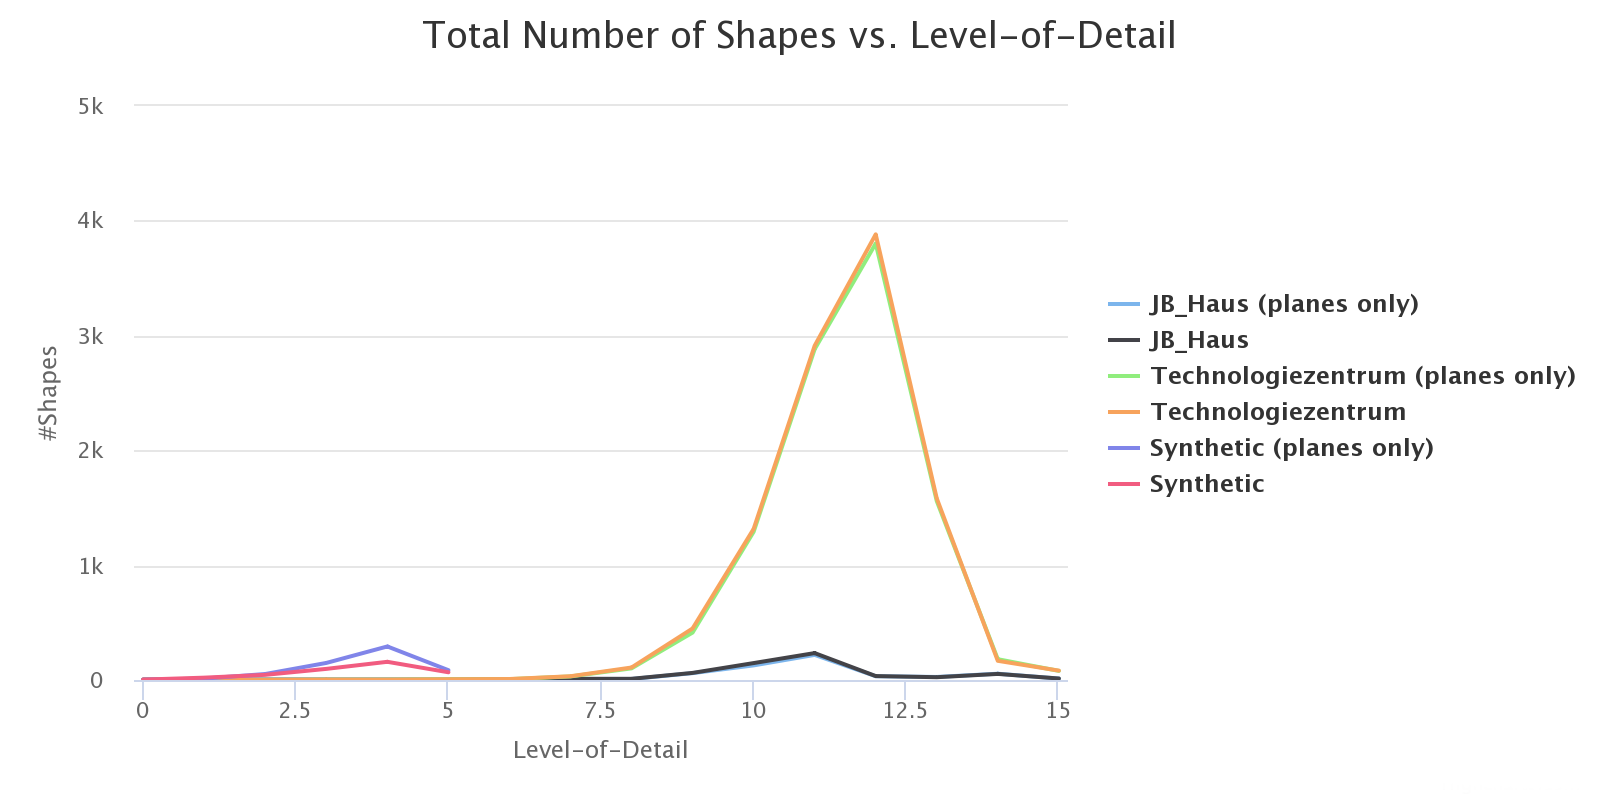
\includegraphics[width=0.8\textwidth]{Results/shapes_total_vs_lod.png}%7
  }\par\medskip
\subcaptionbox{ \label{fig:shapes_averaged_vs_lod}}{%
  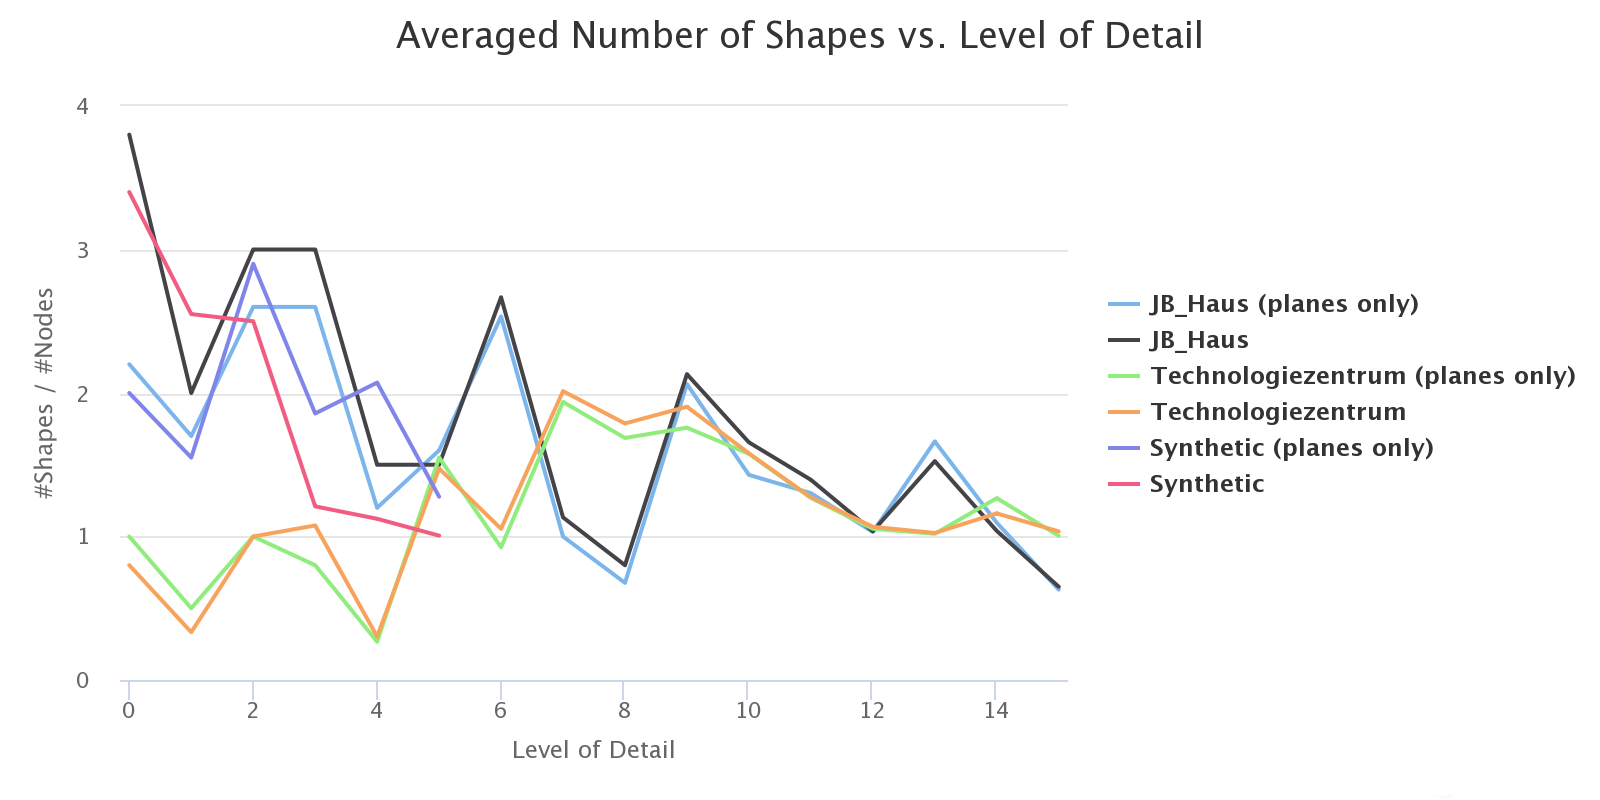
\includegraphics[width=0.8\textwidth]{Results/shapes_averaged_vs_lod.png}%
  }\par\medskip   
\subcaptionbox{ \label{fig:time_vs_lod}}{%
  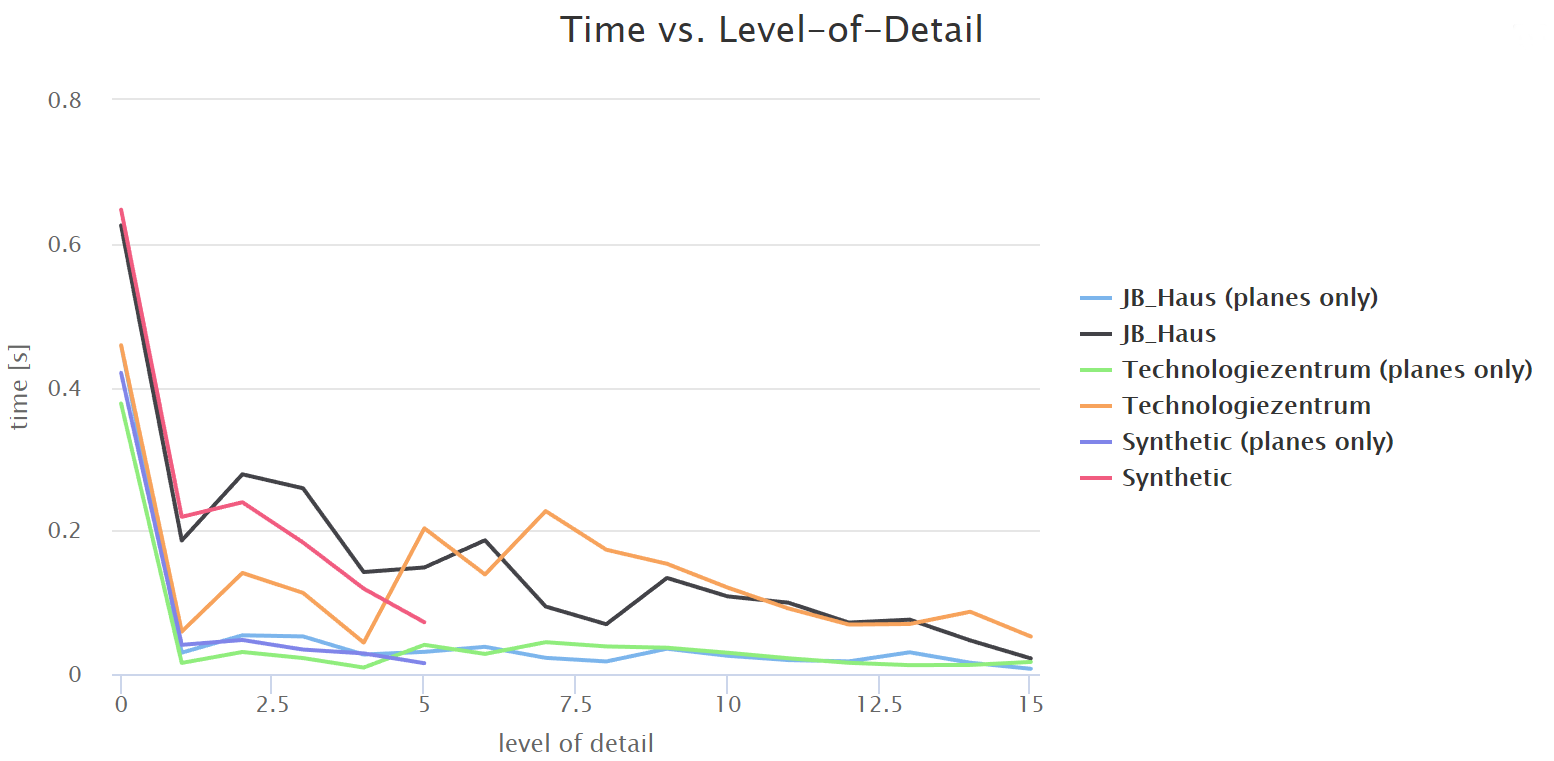
\includegraphics[width=0.8\textwidth]{Results/time_vs_lod.png}%
  } 
\caption[Performance graphs of the interactive shape detection.]
{This set of figures shows different performance measures for the interactive shape detection. All values are averaged over all nodes that share the same level of detail. (a) shows a plot of the total number of shapes vs. the level of detail of the node, (b) shows a plot of the average number of shapes per node vs. the level of detail of the node, and (c) shows a plot of the number of shapes vs. the computation time.}
\label{fig:shape_detection_graphs}
\end{figure}


\section{Shape-Detection Problems and Undesired Behavior}
\label{sec:shape_detection_problems}

A problem with the shape-detection implementation by Schnabel et al. \cite{schnabel-2007-software} are reoccurring non-terminations for some octree nodes, causing the shape-detection coroutine to stall. To circumvent this problem, all shape detection tasks that are dispatched to the \verb|sequential computation applicator| are assigned a timeout value of one second, after which the computation is interrupted. 

\begin{figure}
\centering
\subcaptionbox{ \label{fig:missfittedTorus1}}{%
  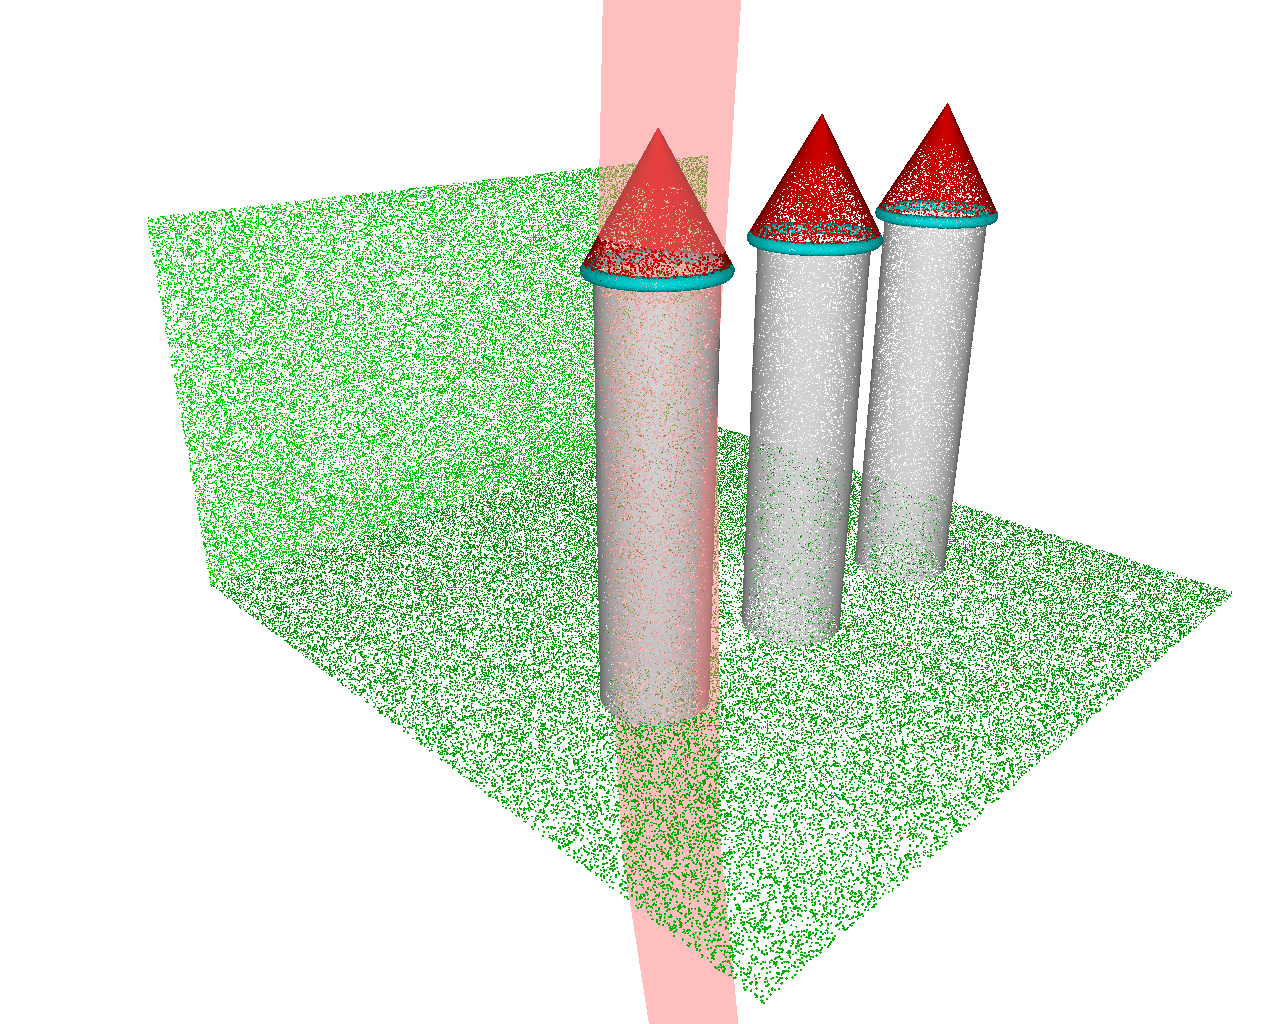
\includegraphics[width=0.425\textwidth]{Results/missfittedTorus1.png}%7
  }%\par\medskip
\subcaptionbox{ \label{fig:missfittedTorus2}}{%
  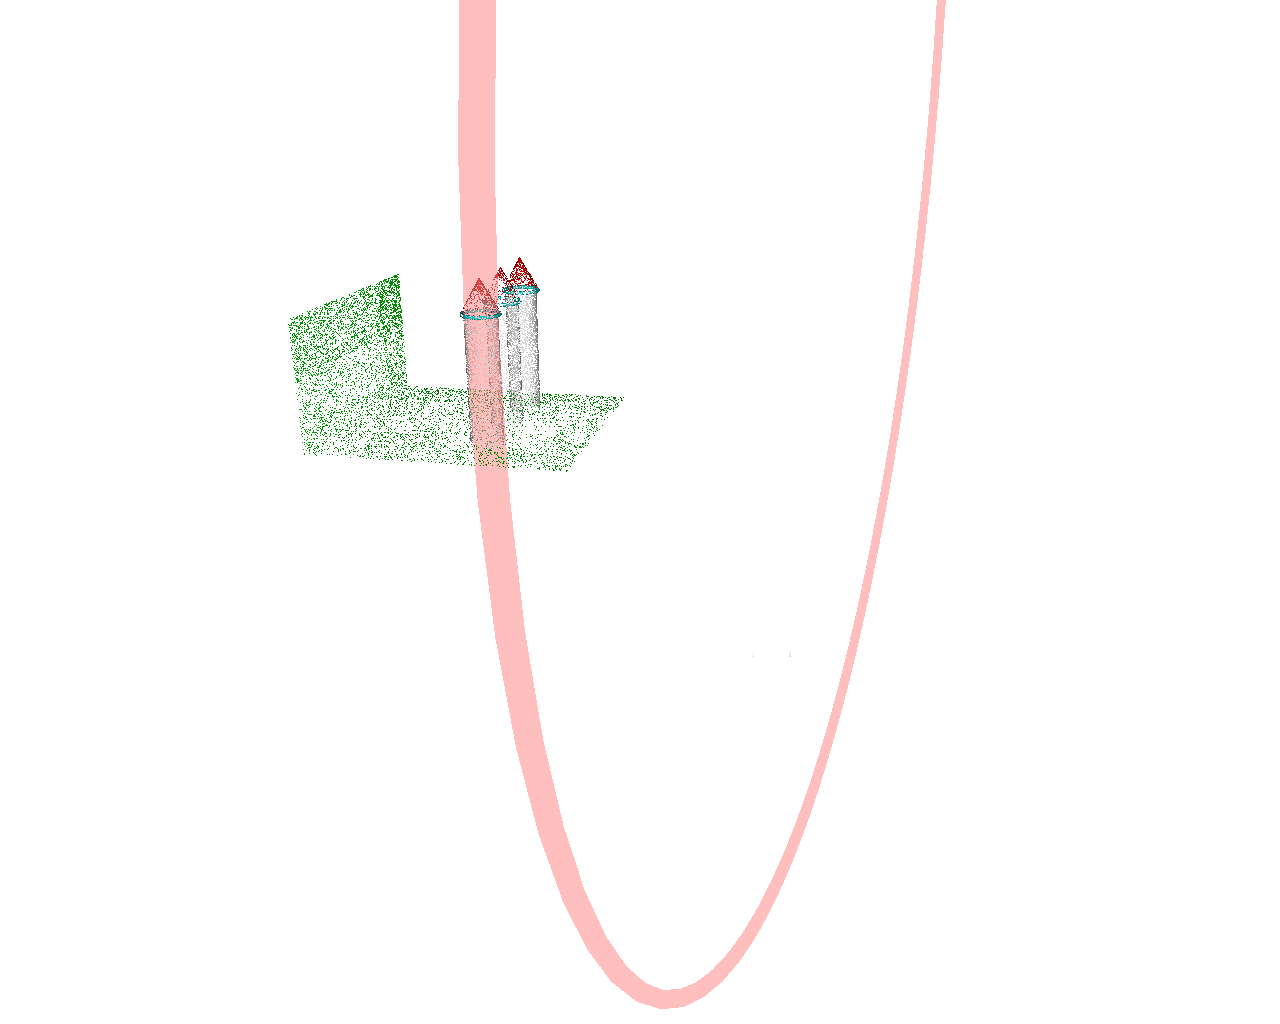
\includegraphics[width=0.425\textwidth]{Results/missfittedTorus2.png}%
  }      
\caption[Implausible torus is detected instead of a more plausible cylinder. ]
{This figure shows a cylinder from the synthetic point cloud whose points are classified as a torus instead of a cylinder. Even though the points fit the torus, determined by the RANSAC options, the result is not plausible, since the user would expect a cylinder for this constellation of points. }
\label{fig:missfittedTorus}
\end{figure}

Another recurring problem with the shape-detection algorithm is the plausibility of detected shapes. The RANSAC options guarantee that shapes are found that fit the local geometry within a certain margin, $\alpha$ for the normal angle and $\epsilon$ for the distance to the shape. So within theses two parameters, the shape is considered to be valid. However, certain constellations of points allow the shape detection to produce results that are accurate in regards to the RANSAC parameters but are implausible to the eye. A prominent example is a torus that is fitted onto a section that describes a cylinder. The major radius of the torus is of such dimensions that the local cylinder fits within the curvature of the torus. Thus, a torus is detected, rather than the simpler cylinder. Figure \ref{fig:missfittedTorus} shows this behavior within an example scene that consists of multiple primitives. Figure \ref{fig:missfittedTorus2} shows the size of the detected torus. 

\par

Such implausible shapes can exist due to the density-controlled $\epsilon$ parameter that weakens the margin for octree nodes of larger volume. Even within a node, the density can vary strongly for different regions. A way to counter this behavior is to create a ranking of the different types of shapes, such that certain types of shapes are detected preferably before other types. A second approach is to check the validity of a detected shape afterward by comparing the dimensions of the detected shape to the extents of the region it was detected in. 


\section{Shape-Detection Results}
\label{sec:shape_detection_results}

Figure \ref{fig:JB_haus_results} and \ref{fig:technologiezentrum_results} compares the results of the RANSAC shape detection on the entire dataset with our interactive approach. Our interactive method finds more shapes that can be grouped into one larger consecutive shape. However, the overall structure of the building is approximated similarly in both techniques as can be seen in (b) and (c) respectively. 

The interactive shape detection was unable to produce results on the synthetic point cloud. On coarse levels of detail, implausible shapes are detected that occluded the entire scene. Hence, a visual comparison of the classic shape detection with our approach did not yield any satisfying results. The results of the classic shape detection for the synthetic scene can be seen in Figure \ref{fig:synthetic_point_cloud_results}


\begin{figure}
\centering
\subcaptionbox{ \label{fig:jb_haus}}{%
  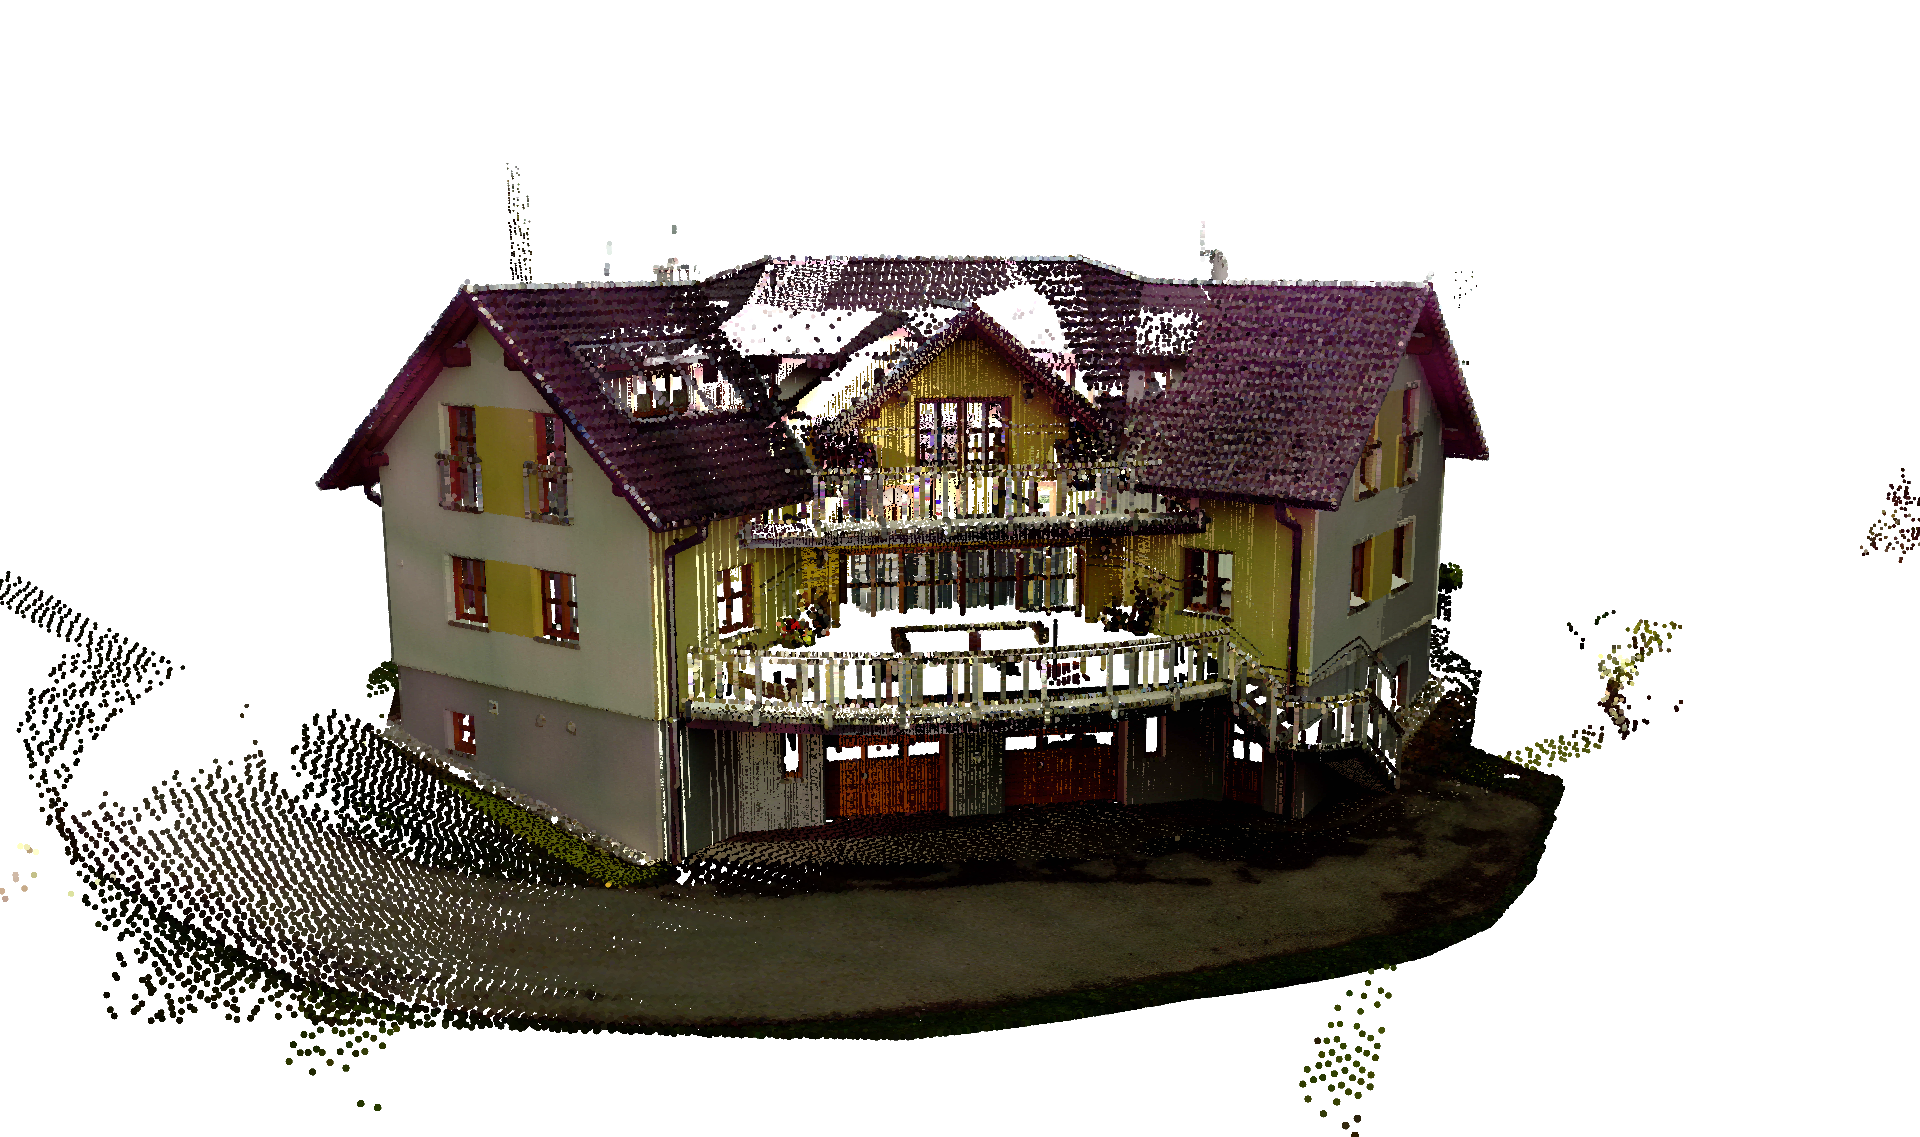
\includegraphics[width=0.7\textwidth]{Results/jb_haus.png}%7
  }
\subcaptionbox{ \label{fig:jb_haus_shapes}}{%
  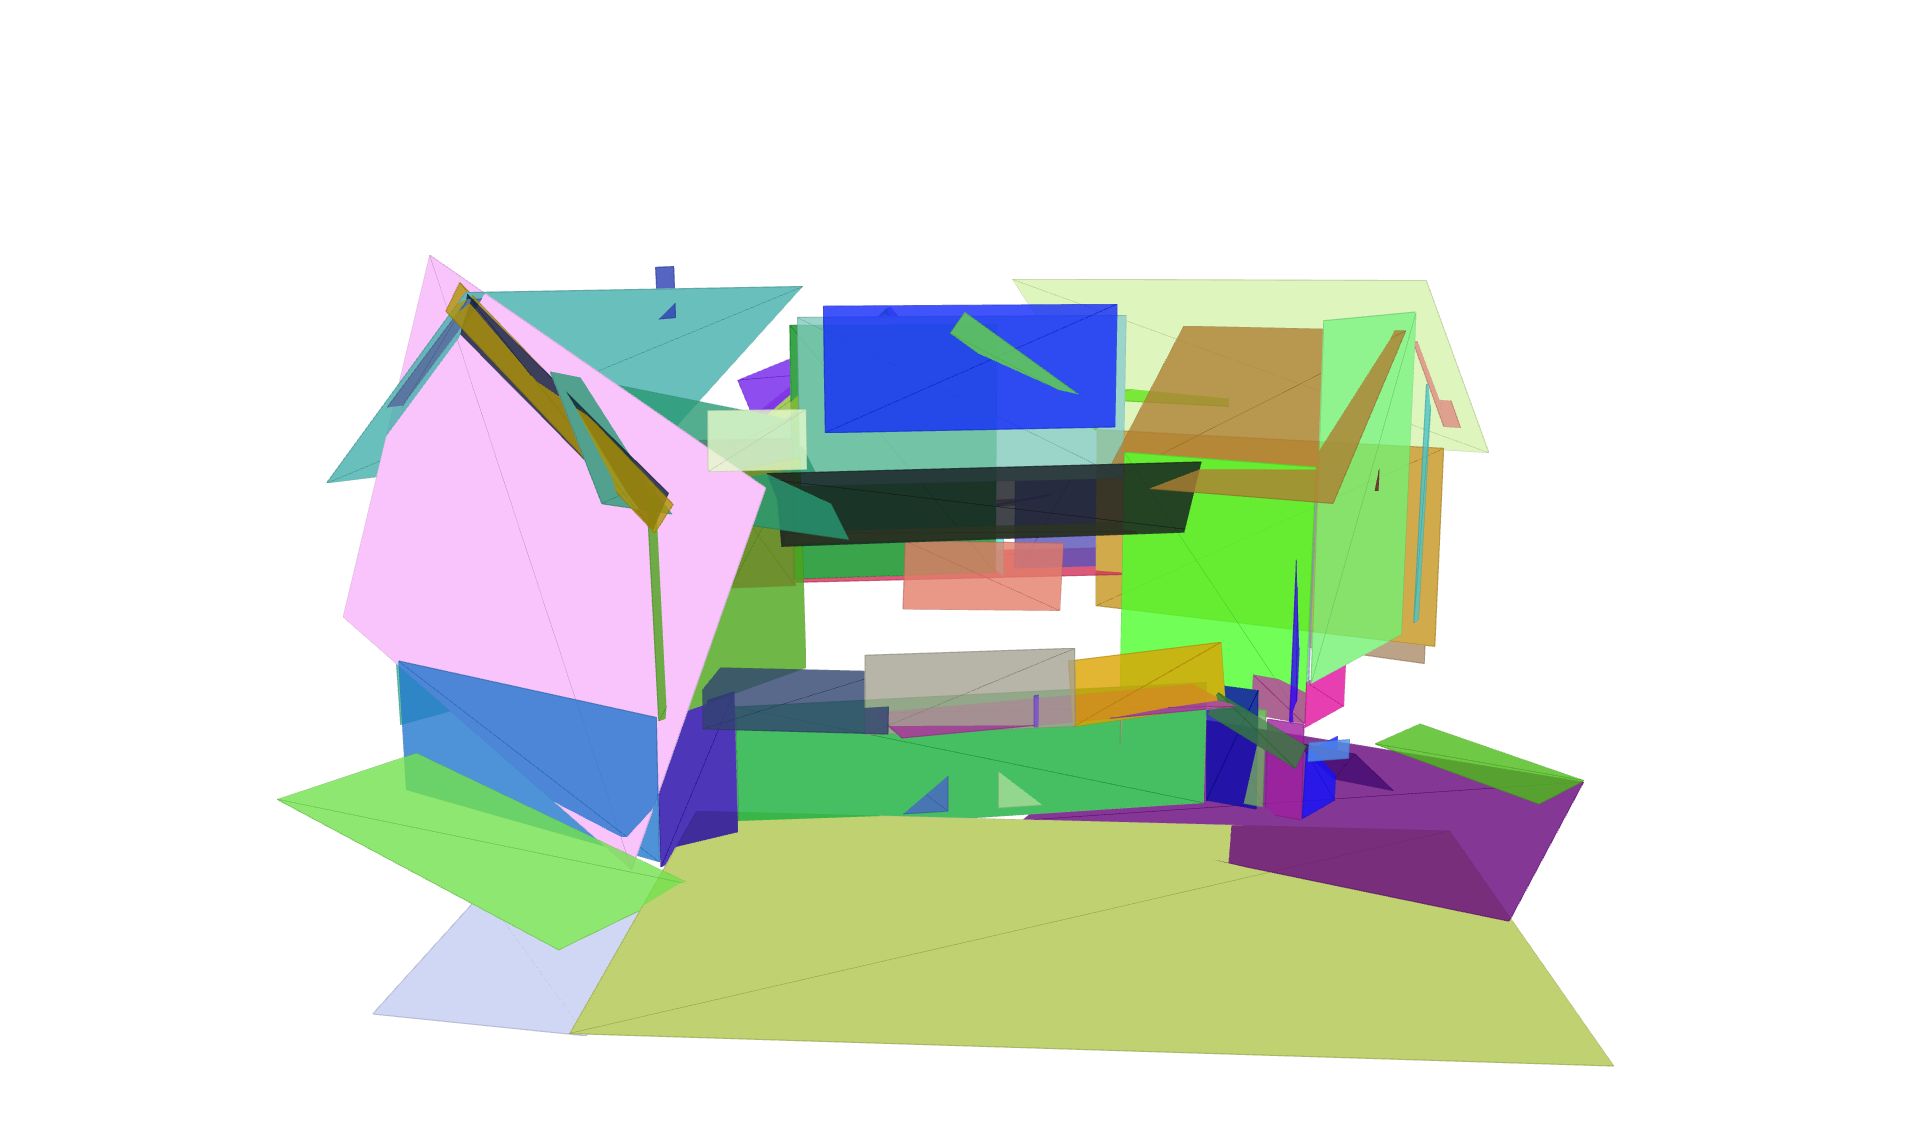
\includegraphics[width=0.7\textwidth]{Results/jb_haus_shapes.png}%
  }
\subcaptionbox{ \label{fig:jb_haus_shapes_interactive}}{%
  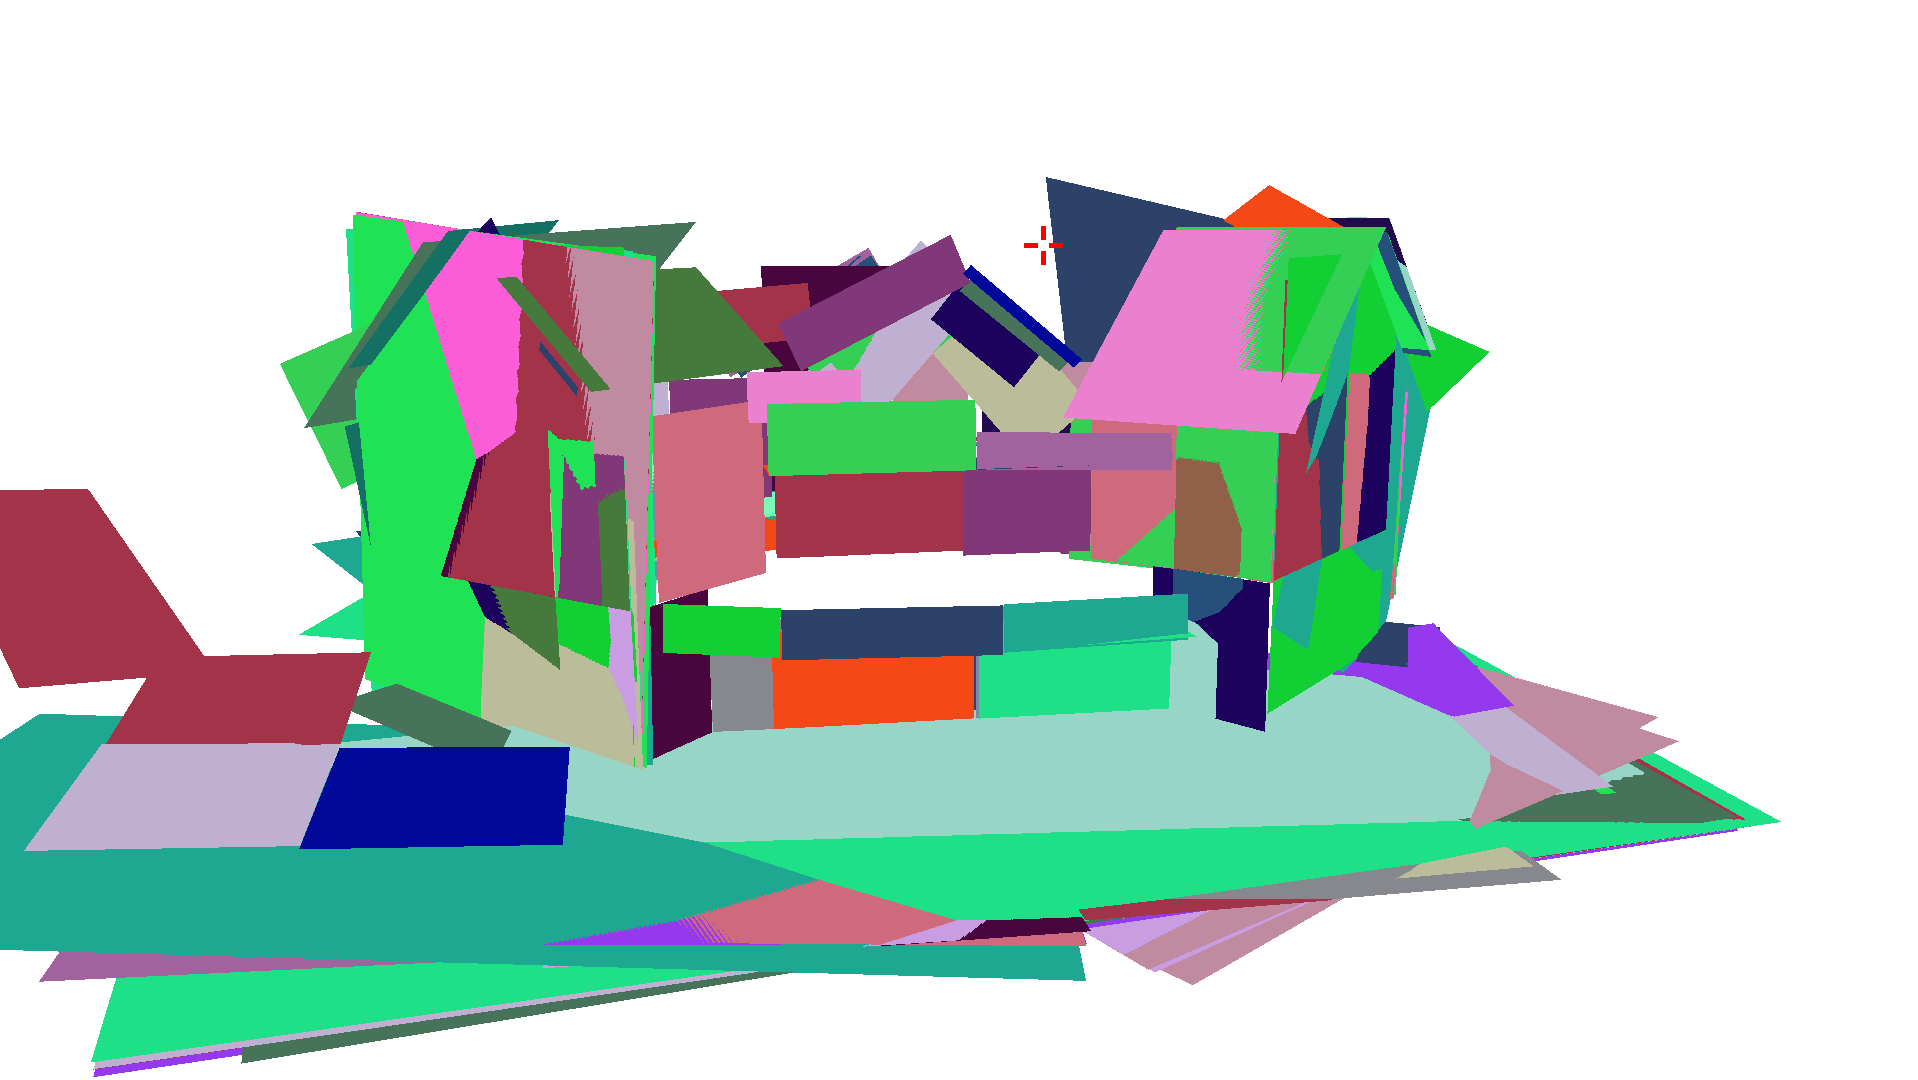
\includegraphics[width=0.7\textwidth]{Results/jb_haus_shapes_interactive.png}%
  }
\caption[Figure (a) shows a rendering of the JB\_haus dataset, (b) shows the resulting shapes of the RANSAC shape detection, (c) shows the result of the interactive shape detection.]
{Figure (a) shows a rendering of the JB\_haus dataset, (b) shows the resulting shapes of the RANSAC shape detection, (c) shows the detected shapes using the interactive shape-detection method.  }
\label{fig:JB_haus_results}
\end{figure}


\begin{figure}
\centering
\subcaptionbox{ \label{fig:technologiezentrum}}{%
  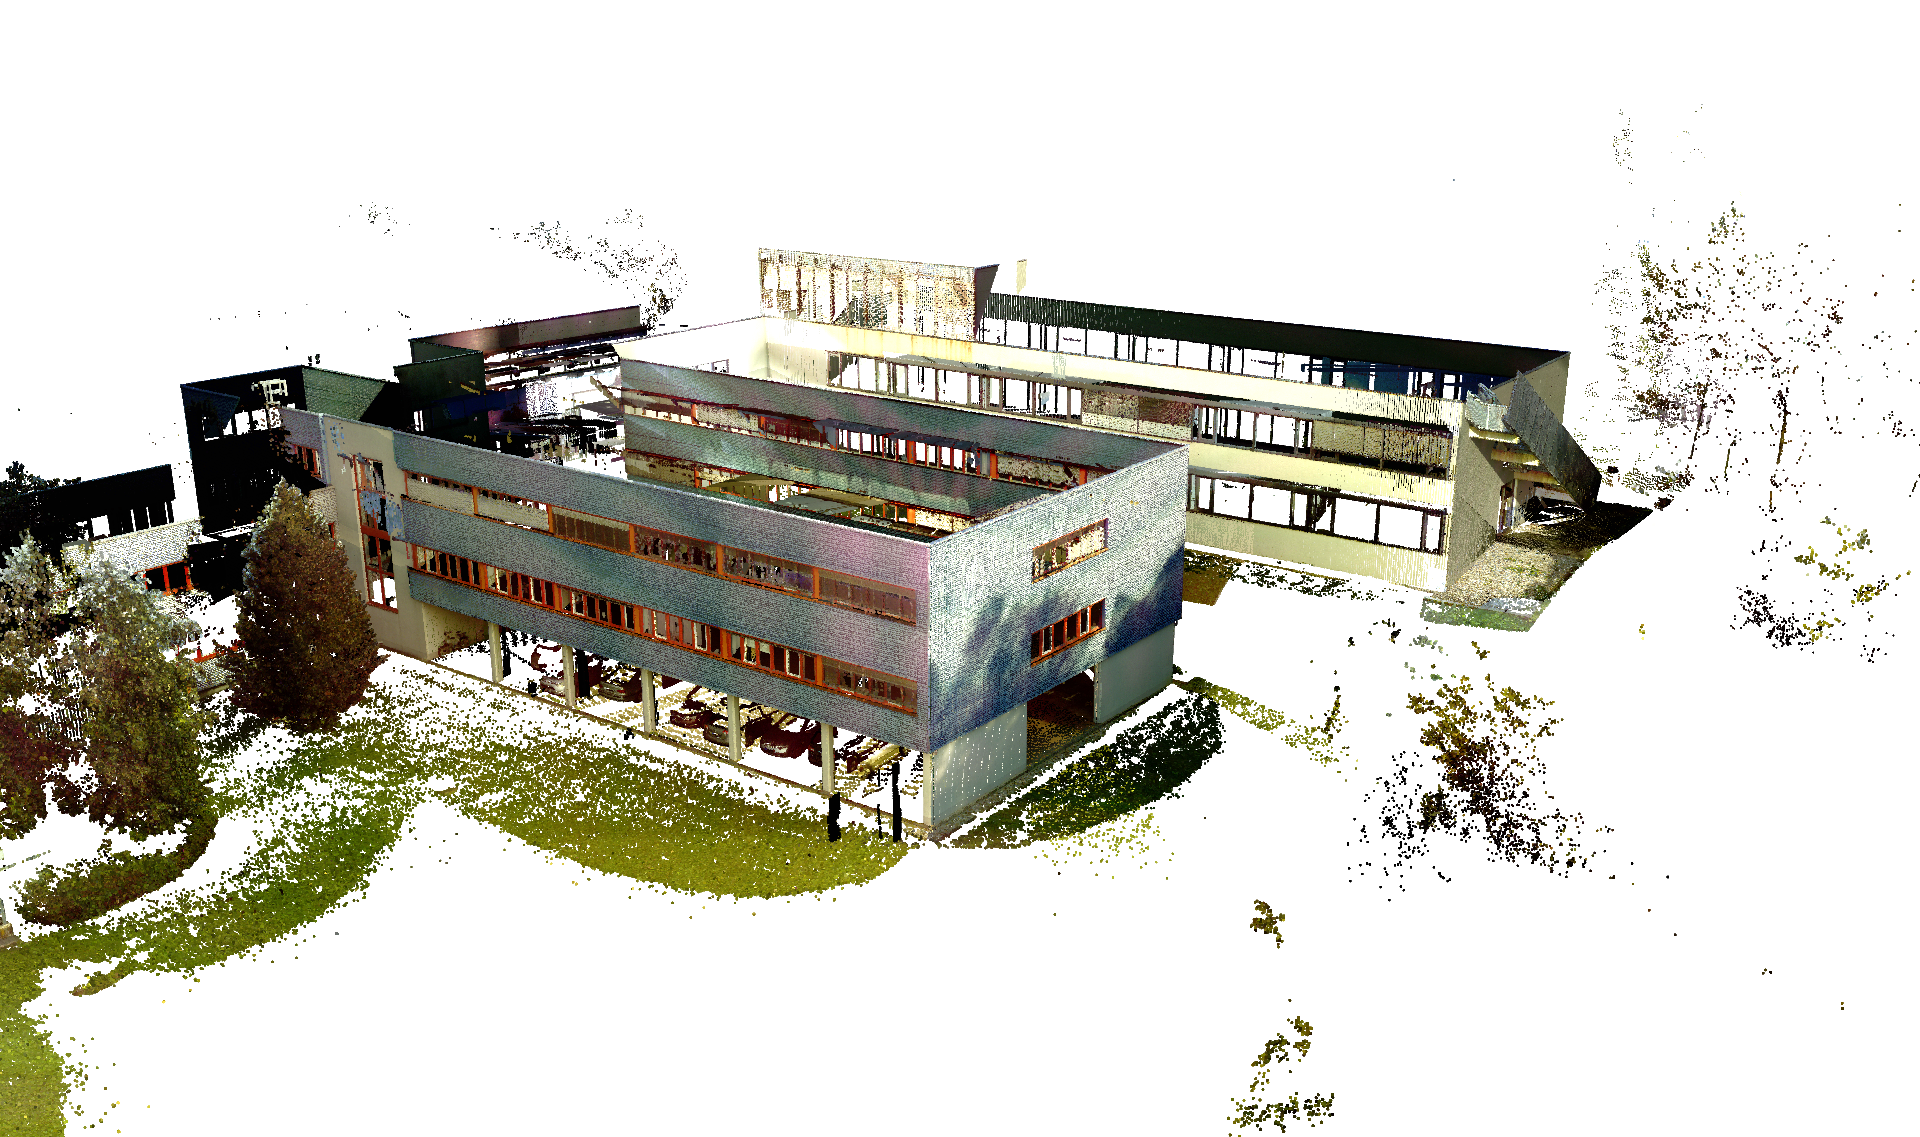
\includegraphics[width=0.7\textwidth]{Results/technologiezentrum.png}%7
  }
\subcaptionbox{ \label{fig:technologiezentrum_shapes}}{%
  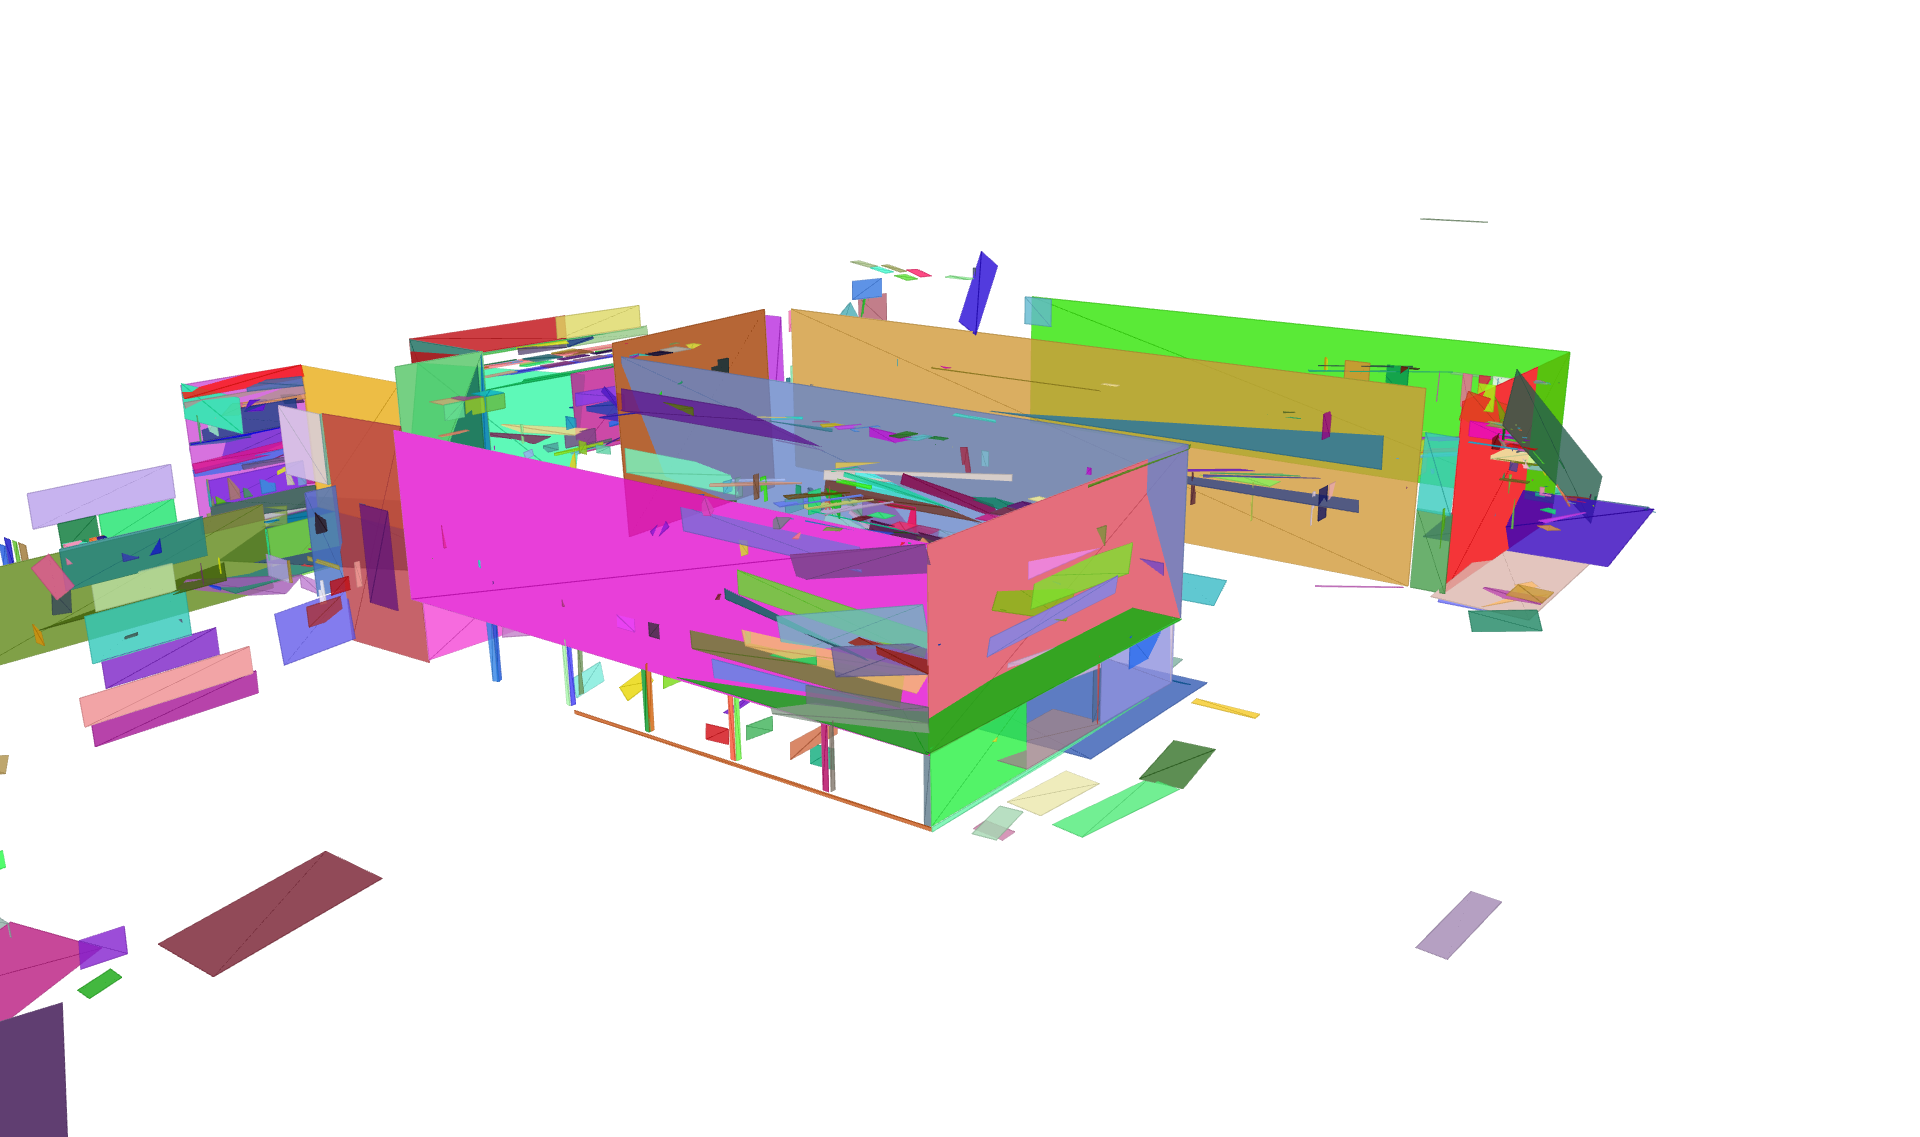
\includegraphics[width=0.7\textwidth]{Results/technologiezentrum_shapes.png}%
  }
\subcaptionbox{ \label{fig:technologiezentrum_shapes_interactive}}{%
  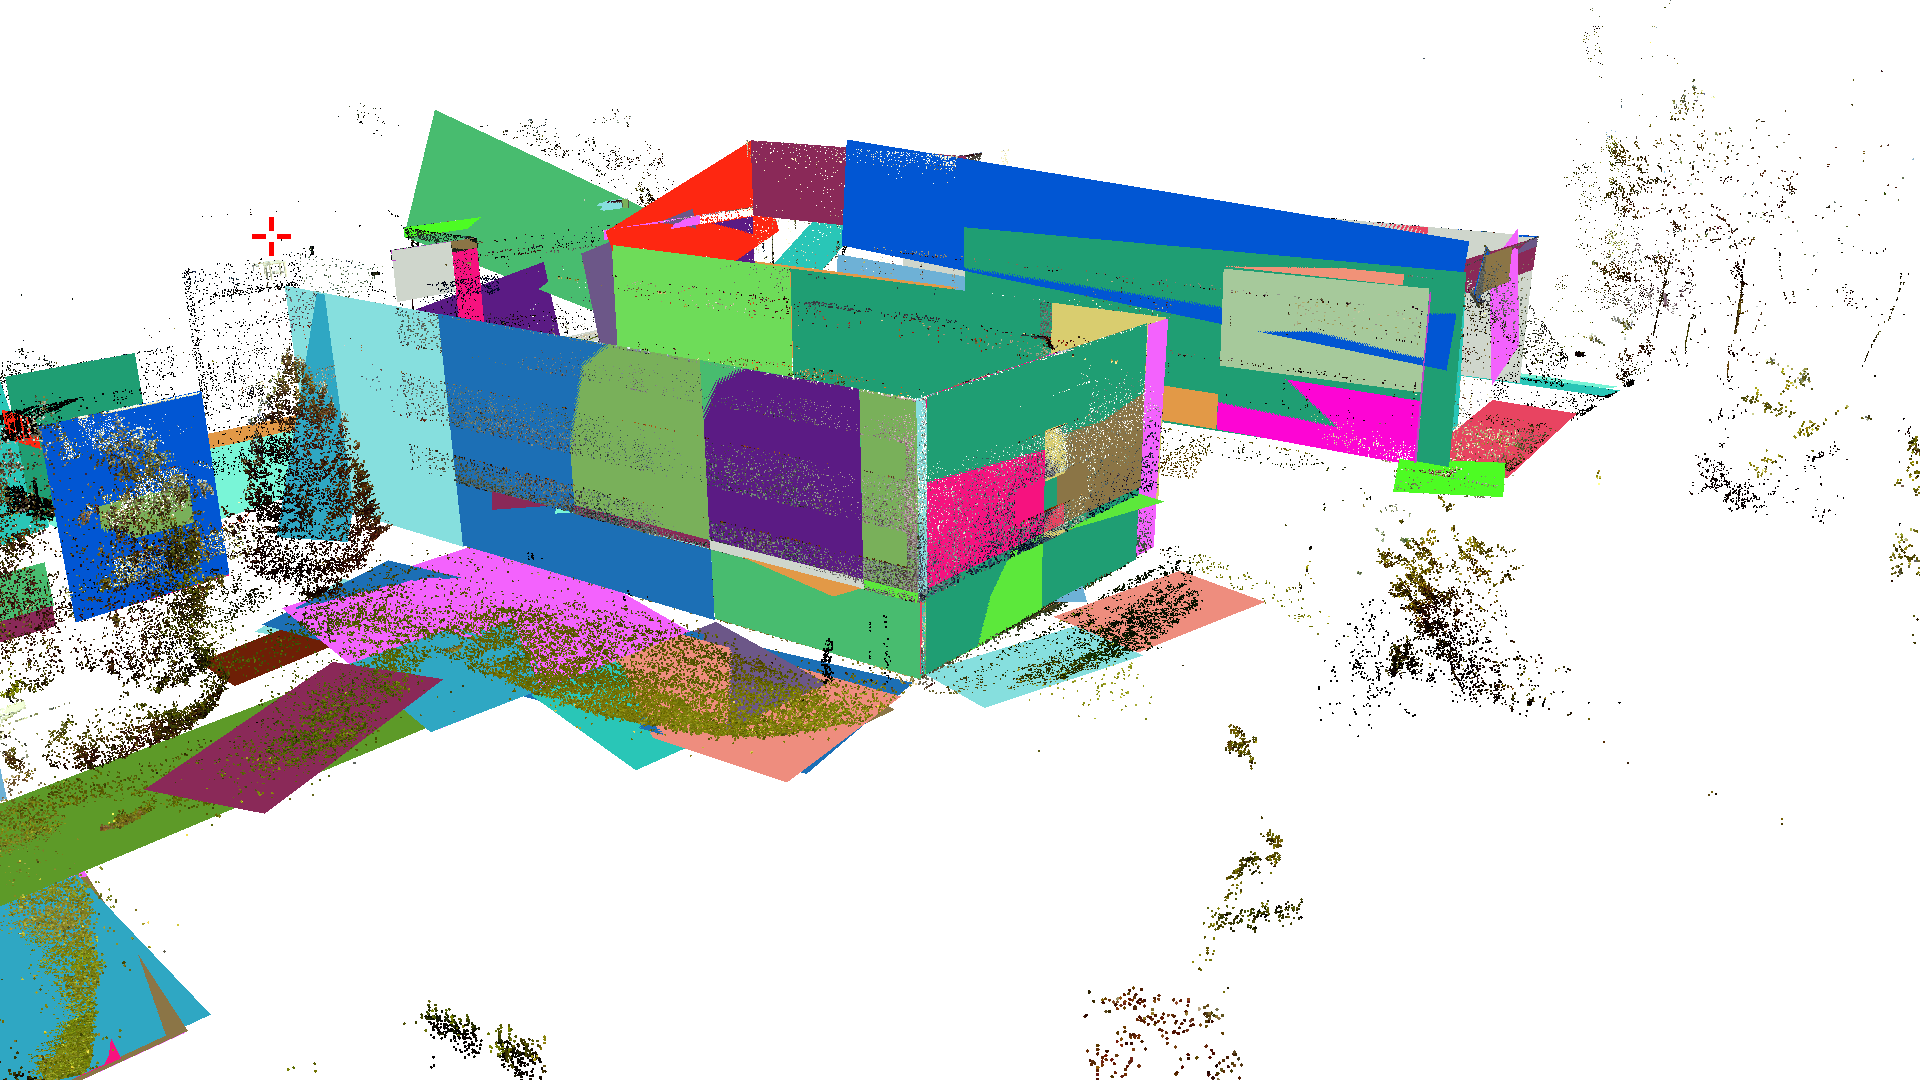
\includegraphics[width=0.7\textwidth]{Results/technologiezentrum_shapes_interactive.png}%
  }
\caption[Figure (a) shows a rendering of the Technologiezentrum dataset, (b) shows the resulting shapes of the RANSAC shape detection, (c) shows the result of the interactive shape detection.]
{Figure (a) shows a rendering of the Technologiezentrum dataset, (b) shows the resulting shapes of the RANSAC shape detection, (c) shows the detected shapes using the interactive shape-detection method.}
\label{fig:technologiezentrum_results}
\end{figure}


\begin{figure}[p]
\centering
\subcaptionbox{ \label{fig:synthetic_point_cloud}}{%
  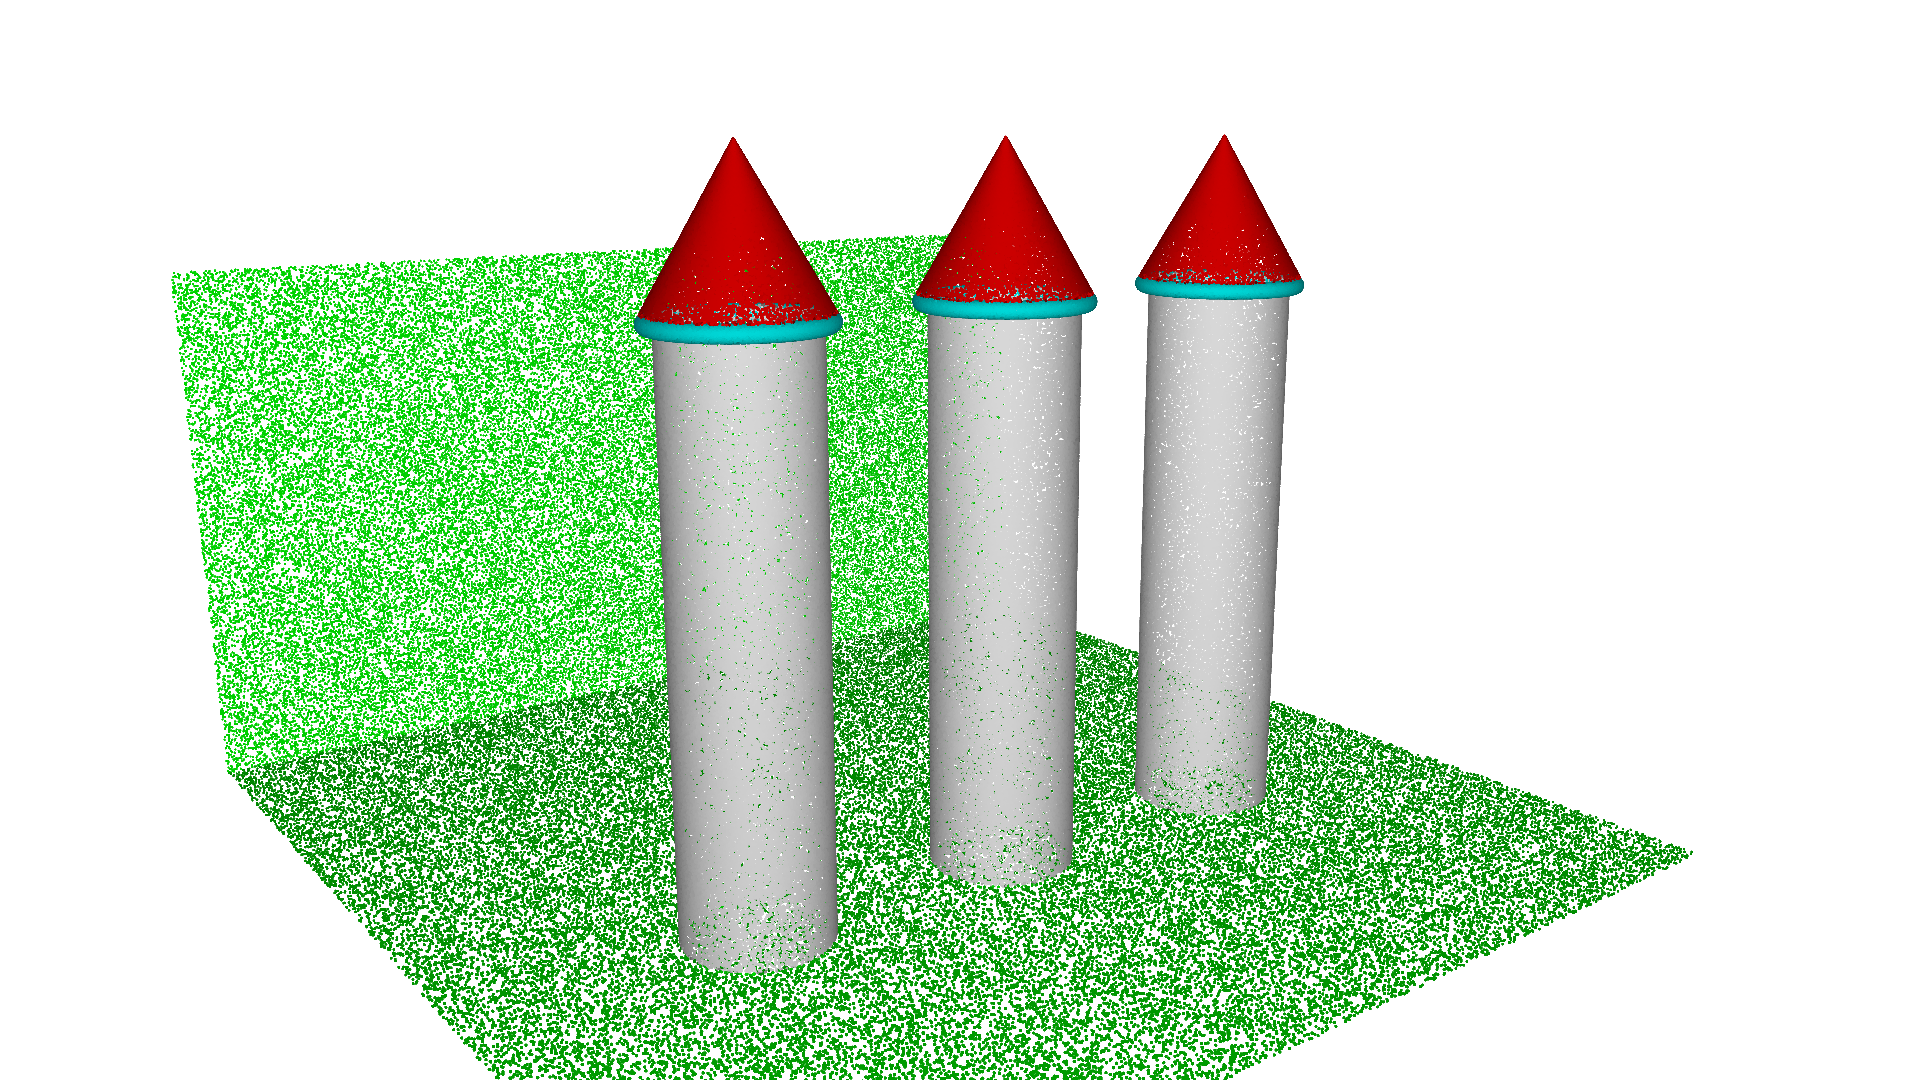
\includegraphics[width=0.7\textwidth]{Results/synthetic_point_cloud.png}%7
  }
\subcaptionbox{ \label{fig:synthetic_point_cloud_shapes}}{%
  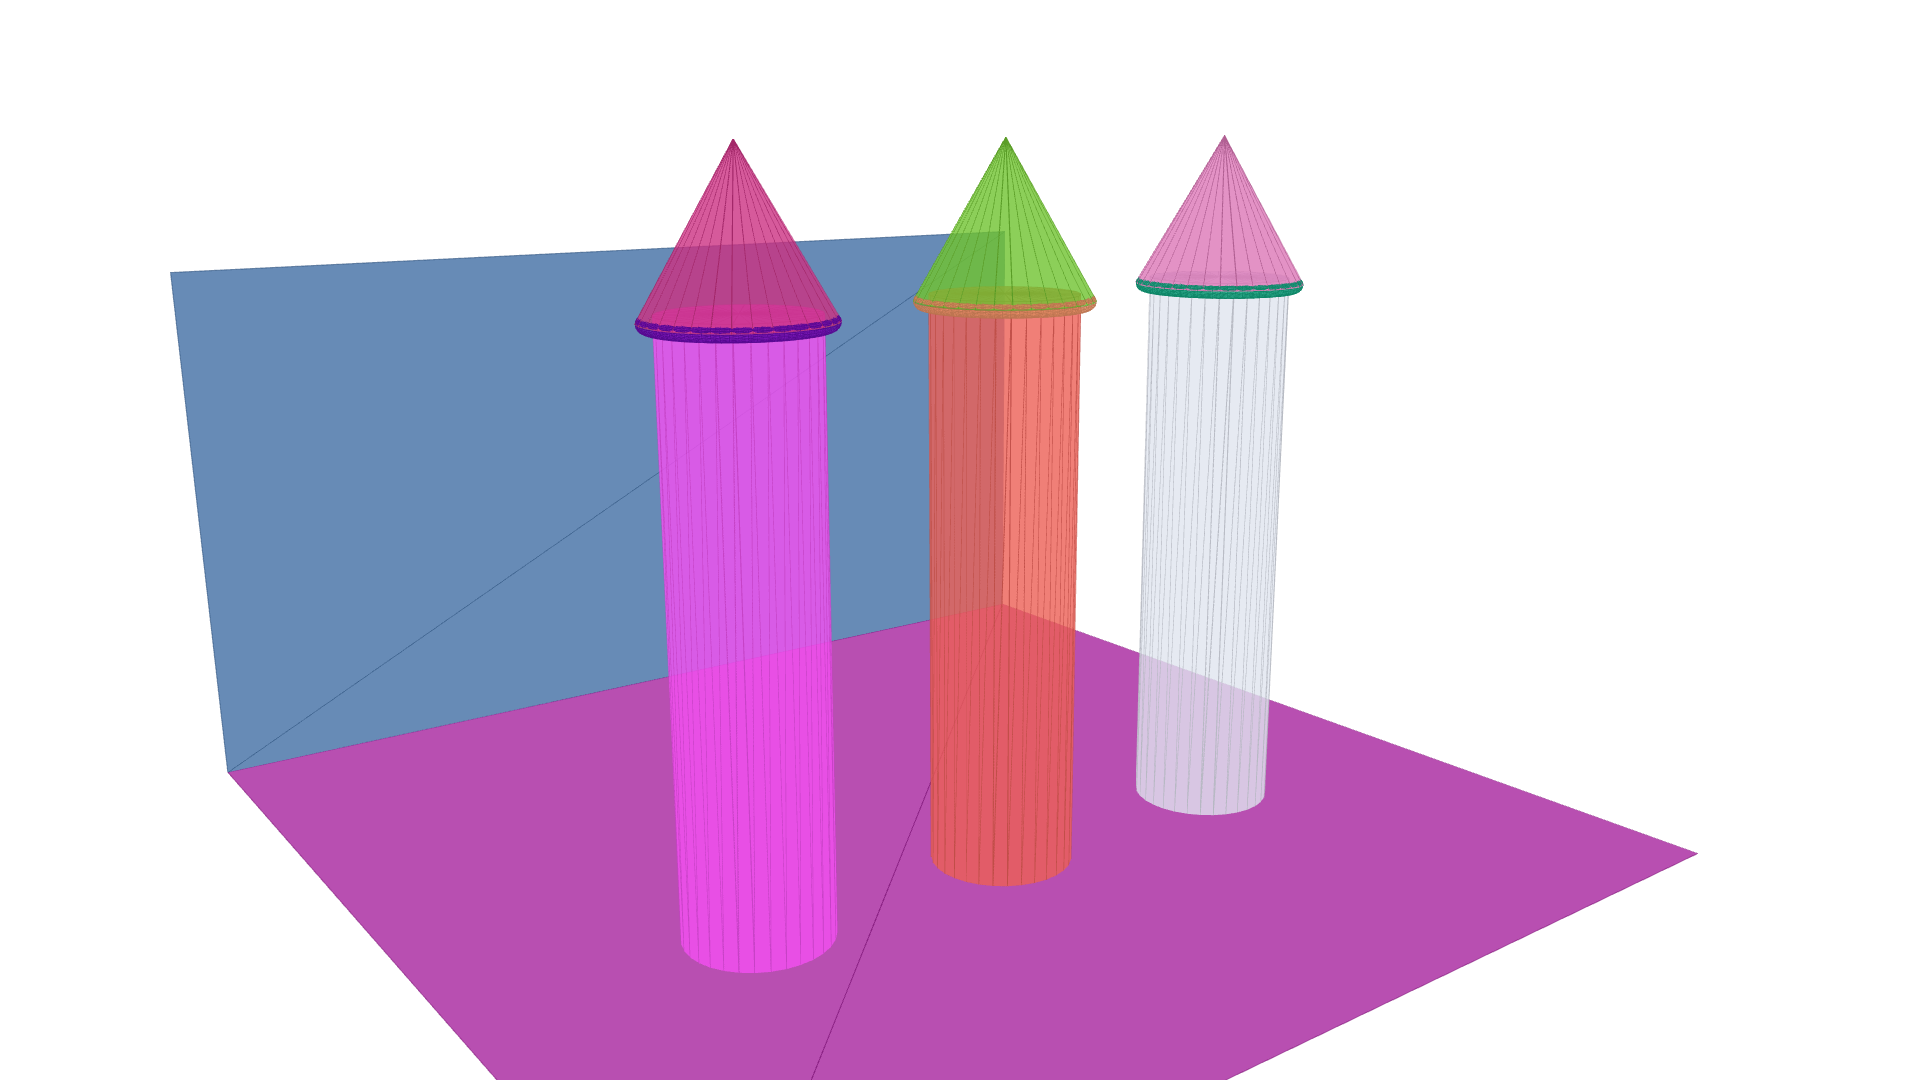
\includegraphics[width=0.7\textwidth]{Results/synthetic_point_cloud_shapes.png}%
  }
\caption[Rendering of the synthetic point cloud in (a), rendering of the detected shapes in (b)]
{(a) shows the synthetic point cloud, consisting of two planes, three cylinders, three tori, and three cones. (b) shows the detected shapes rendered as triangle meshes. For each shape in the point cloud, the RANSAC shape detection has found a suitable primitive shape. }
\label{fig:synthetic_point_cloud_results}
\end{figure}


\section{Interaction Performance}
\label{sec:interaction_performance}

The use of support shapes for assisted interaction improves the computation time. \textit{Shape-assisted point picking} is tested against traditional point picking. Point picking is performed only on points that are visible to the user. Hence, the size of the point cloud does not affect the picking performance. However, the level-of-detail culling does. The results in Table \ref{tab:picking_performance} are obtained by randomly picking points with and without support shape on all three datasets. Over all datasets, shape-assisted point picking performs better than traditional point picking. For shape-assisted point picking, the actual per-point processing time is higher due to the additional point-shape relation check. However, the assisted interaction performs significantly better due to the reason that traditional point picking must process a larger set of octree nodes (i.e., all nodes that intersect the pick ray), whereas shape-assisted point picking only needs to check nodes that intersect the support shape. 

\begin{table}[b]
\centering
\begin{tabular}{ l|r| r | r }
                       &\multicolumn{3}{c}{\textbf{Time (ms)}}\\
                       & \textbf{min}    & \textbf{max}    & \textbf{avg} \\
        \hline
        Without support& 13.402100  & 148.346100 & 37.964309 \\
        With support   &  0.348200  &  39.929400 &  3.281752 \\

\end{tabular}
\caption{This table showcases the benchmark results for point picking with and without the use of a support shape. The assisted technique performs on average more than ten times faster than traditional point picking. }
\label{tab:picking_performance}
\end{table}

The lasso selection is performed on the entire point cloud. Hence, the size of the point cloud directly influences the response time of the interaction. Furthermore, the size and form of a lasso also affect the computation time. For a rectangular selection, it takes significantly less time to compute the intersection with a point than for a more complex polygon. The shape-assisted lasso selection is benchmarked by directly comparing the computation time to a classical lasso selection that shares the same lasso polygon. The performance measures in Table \ref{tab:lasso_performance} are obtained from selection on all datasets.

\begin{table}
\centering
\begin{tabular}{ l | r | r | r }
                   & \multicolumn{3}{c}{\textbf{Time (ms)}}\\
                   & \textbf{min}    & \textbf{max}    & \textbf{avg} \\
        \hline
Without support    & 193.628900 & 2494.494800 & 748.725405 \\
With support       & 191.082600 & 923.332500 & 437.933686 \\

\end{tabular}
\caption{This table showcases the benchmark results for shape-assisted lasso selection compared to traditional lasso selection. On average, shape-assisted lasso selection performs faster. However, performance strongly depends on the size of the point cloud and selection. }
\label{tab:lasso_performance}
\end{table}

The testing methodology for the lasso selection was to perform the shape-assisted and the traditional lasso selection for the same lasso polygon. Hence, the testing provided a direct comparison of the interactions for the same lasso and the same point cloud. We calculated the ratio between the processing times of both techniques. We obtained an averaged ratio between the shape-assisted and traditional lasso selection of $\sim$1.81, meaning that the traditional lasso selection takes on average approximately $1.8$ times as long to compute as the shape-assisted lasso selection. 


\section{Interaction Results}
\label{sec:interaction_results}

This section presents a set of figures that showcase the different interactions from Section \ref{sec:interactions}. Examples of all interactions using the JB\_Haus dataset are presented already throughout this thesis. This section shows the results for the interactions on both the Technologiezentrum and the synthetic dataset. The synthetic dataset showcases the use of non-planar support shapes for the assisted interactions. 

Figures \ref{fig:technologiezentrum_lasso}, \ref{fig:technologiezentrum_brush}, and \ref{fig:technologiezentrum_lod_increment} show examples of a shape-assisted lasso selection, volumetric-brush selection and level-of-detail increment using a support shape on the Technologiezentrum dataset. 

Figures \ref{fig:synthetic_scene_lasso} and \ref{fig:synthetic_scene_brush} show a shape-assisted lasso selection and volumetric-brush selection. The support shape is a cylinder. While the volumetric brush still only follows the surface of the cylinder, the lasso selects partly 'through' the point set, more precisely, the lasso selection is performed on points on the back side of the cylinder as well. 

%\begin{figure}
%\centering
%\subcaptionbox{ \label{fig:technologiezentrum_interactive_shape_detection1}}{%
%  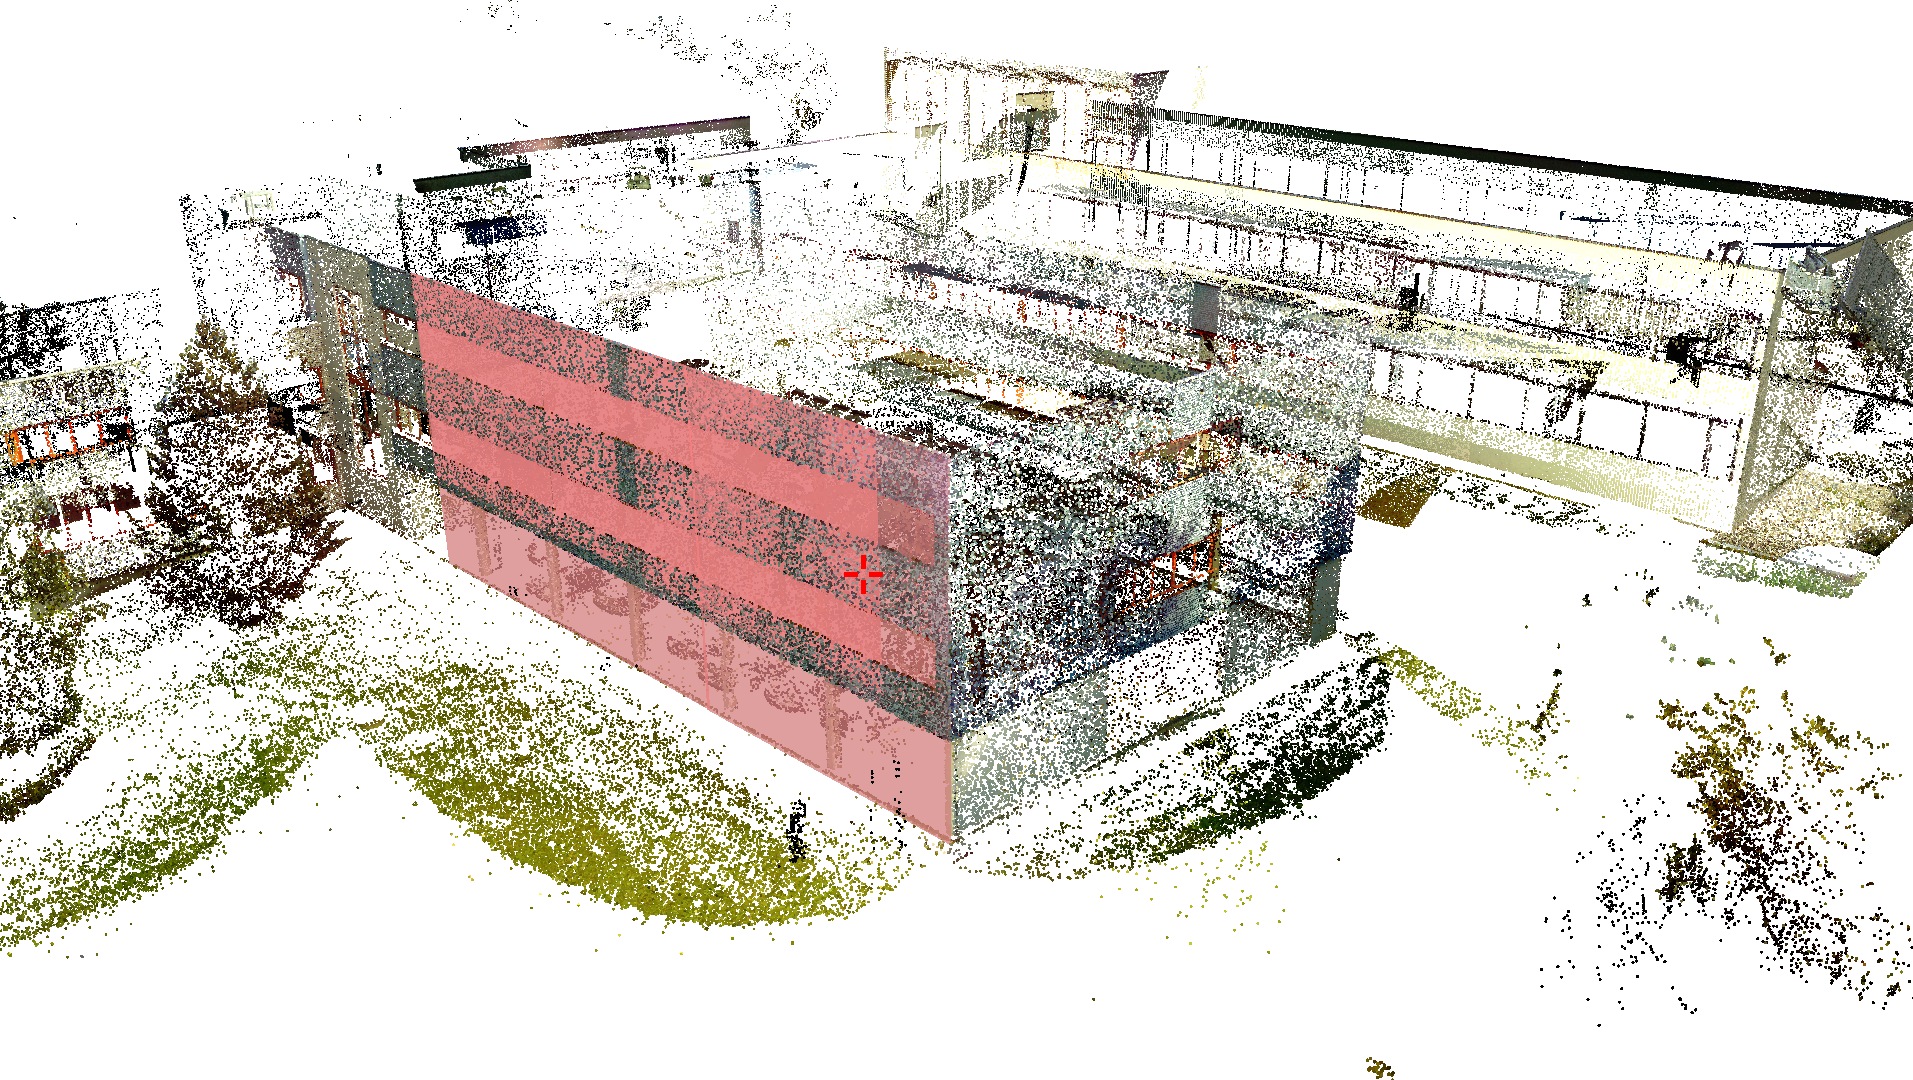
\includegraphics[width=\textwidth]{Results/technologiezentrum_interactive_shape_detection1.png}%7
%  }
%\subcaptionbox{ \label{fig:technologiezentrum_interactive_shape_detection2}}{%
%  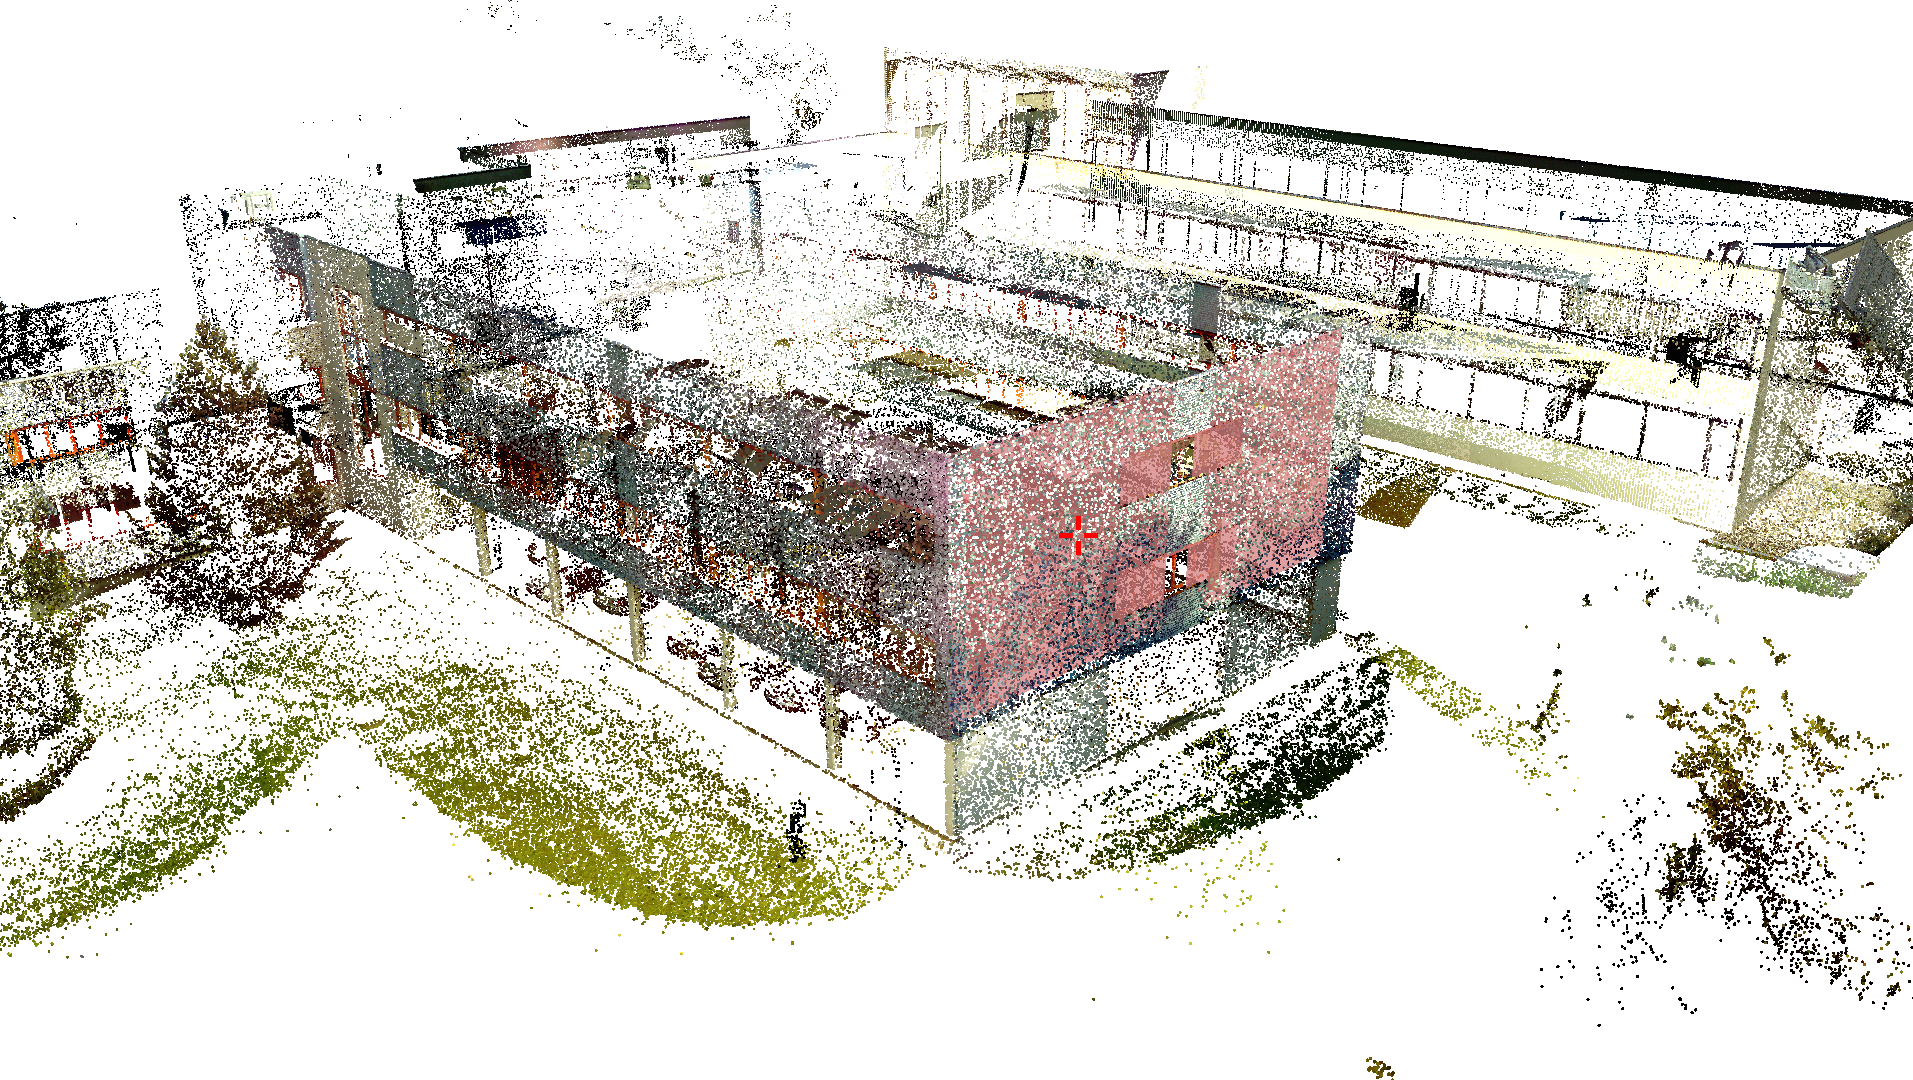
\includegraphics[width=\textwidth]{Results/technologiezentrum_interactive_shape_detection2.png}%
%  }
%\caption[Two examples of user-guided shape detection]
%{This figure shows a rendering of the Technologiezentrum dataset. Based on the cursor position (indicated as the red cross hair) a different shape is selected. The %shape is rendered in red. (a) and (b) show different shapes for different parts of the point cloud. Both shapes are a part of a wall.}
%\label{fig:technologiezentrum_interactive_shape_detection}
%\end{figure}

\begin{figure}[h]
\centering
\subcaptionbox{ \label{fig:technologiezentrum_lasso1}}{%
  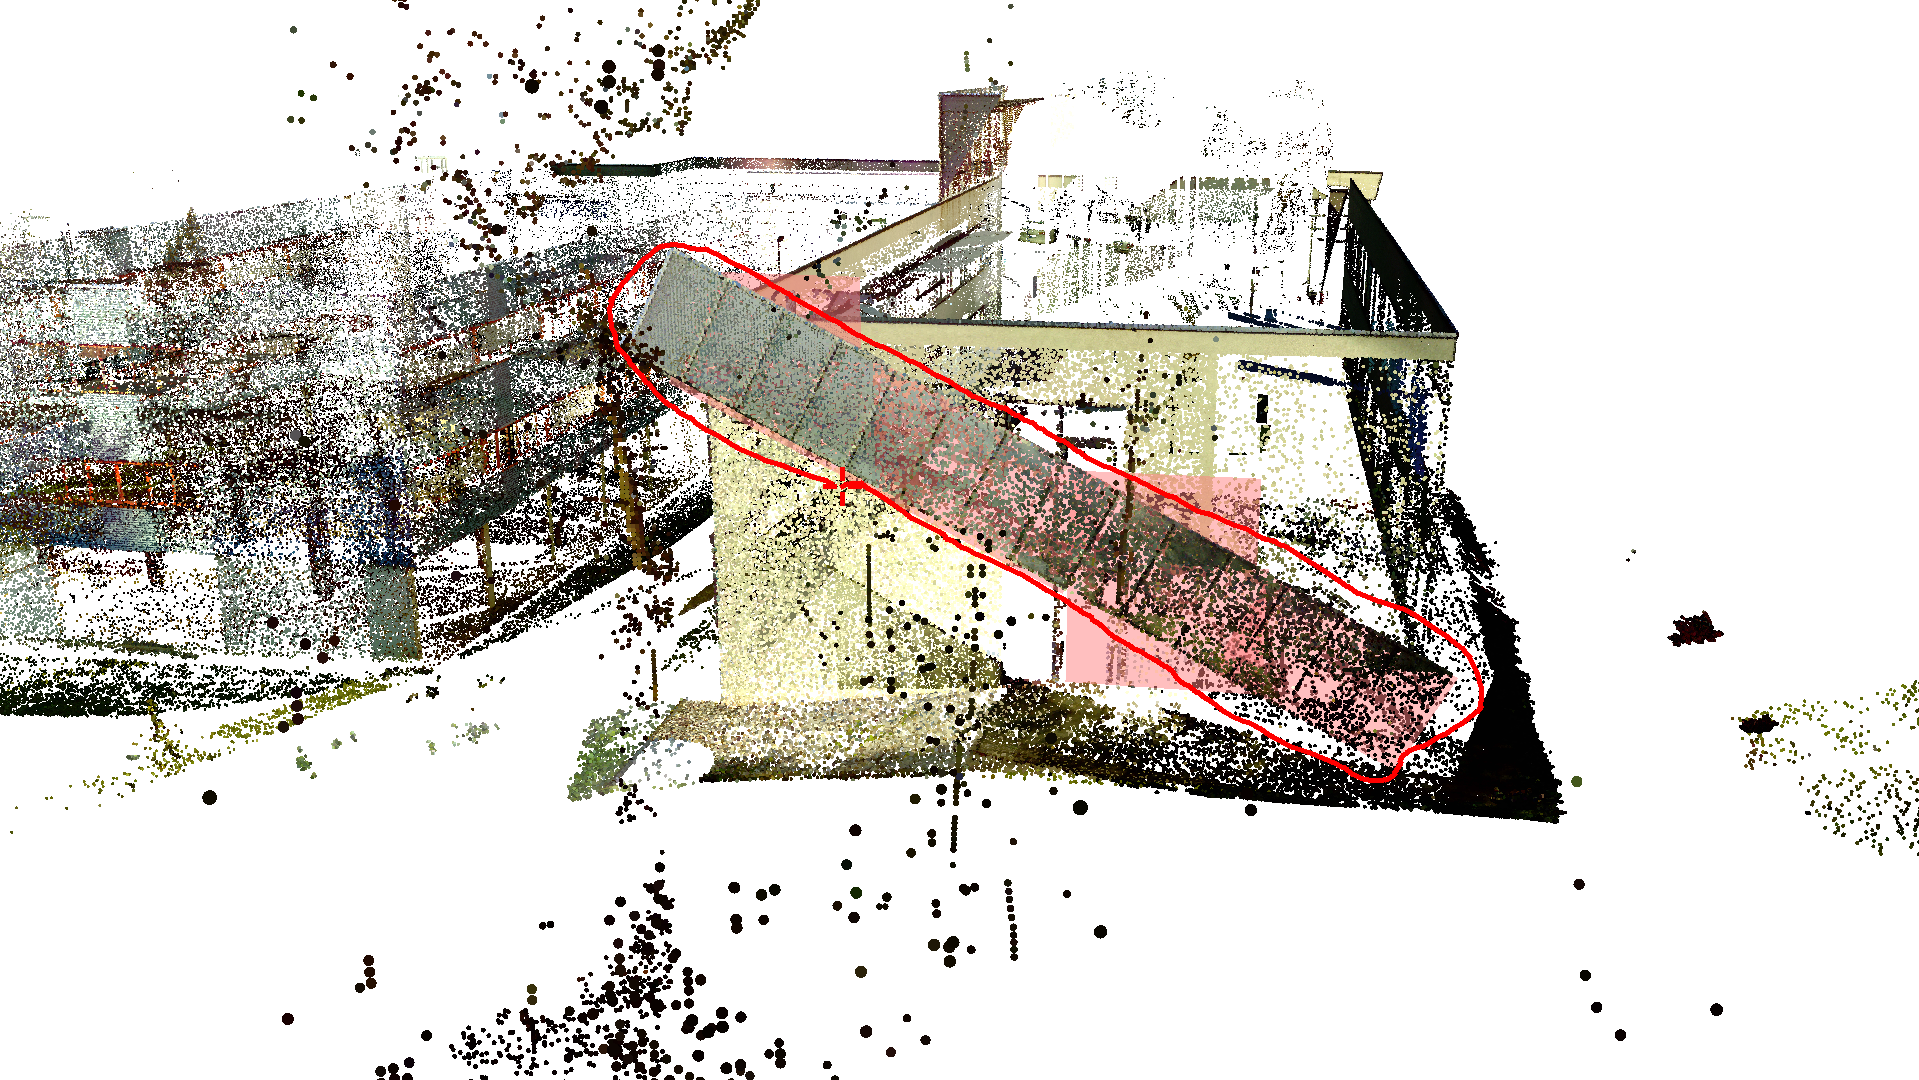
\includegraphics[width=0.9\textwidth]{Results/technologiezentrum_lasso1.png}%7
  }
\subcaptionbox{ \label{fig:technologiezentrum_lasso2}}{%
  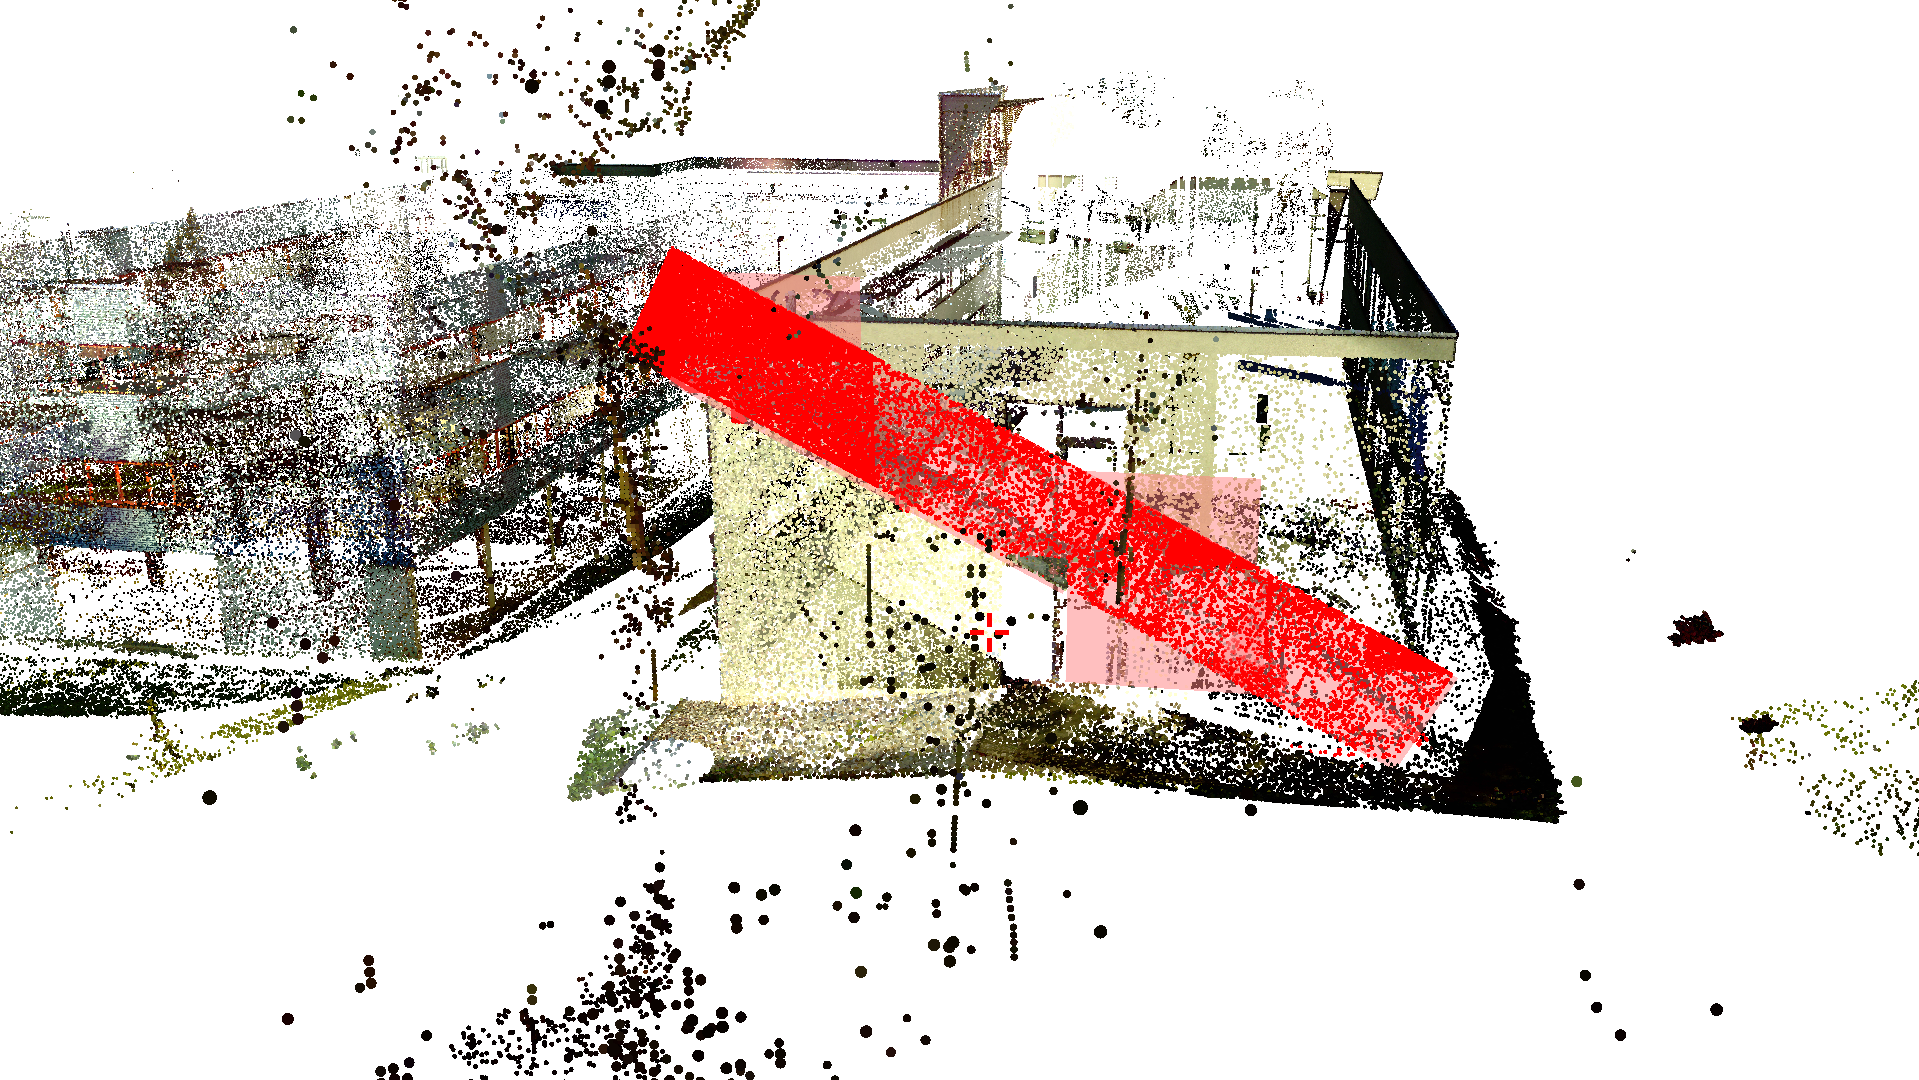
\includegraphics[width=0.9\textwidth]{Results/technologiezentrum_lasso2.png}%
  }
\caption[Example of an improved lasso selection]
{A lasso selection is performed on the selected support shape in (a). Only points are selected that lie on the support shape as shown in (b). Points in front and back of the support shape are not selected. }
\label{fig:technologiezentrum_lasso}
\end{figure}


\begin{figure}
\centering
\subcaptionbox{ \label{fig:technologiezentrum_brush1}}{%
  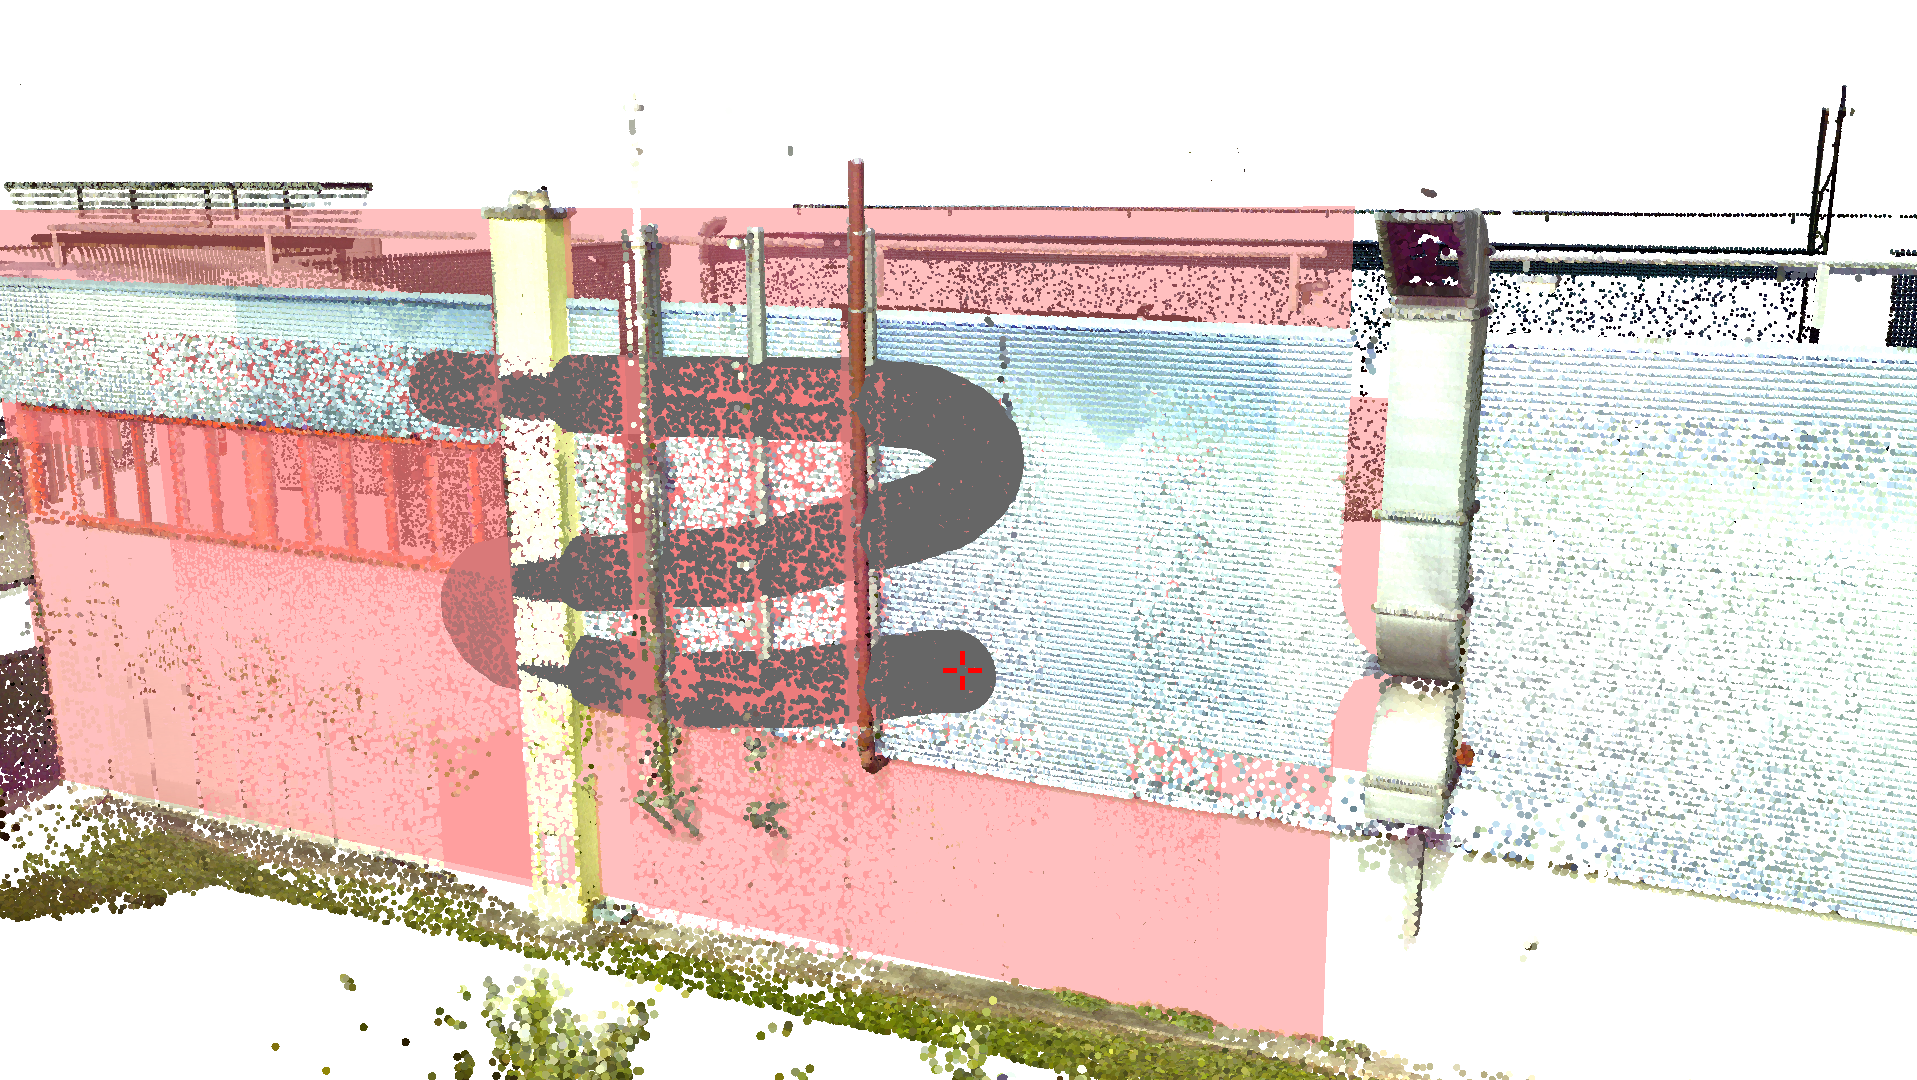
\includegraphics[width=\textwidth]{Results/technologiezentrum_brush1.png}%7
  }
\subcaptionbox{ \label{fig:technologiezentrum_brush2}}{%
  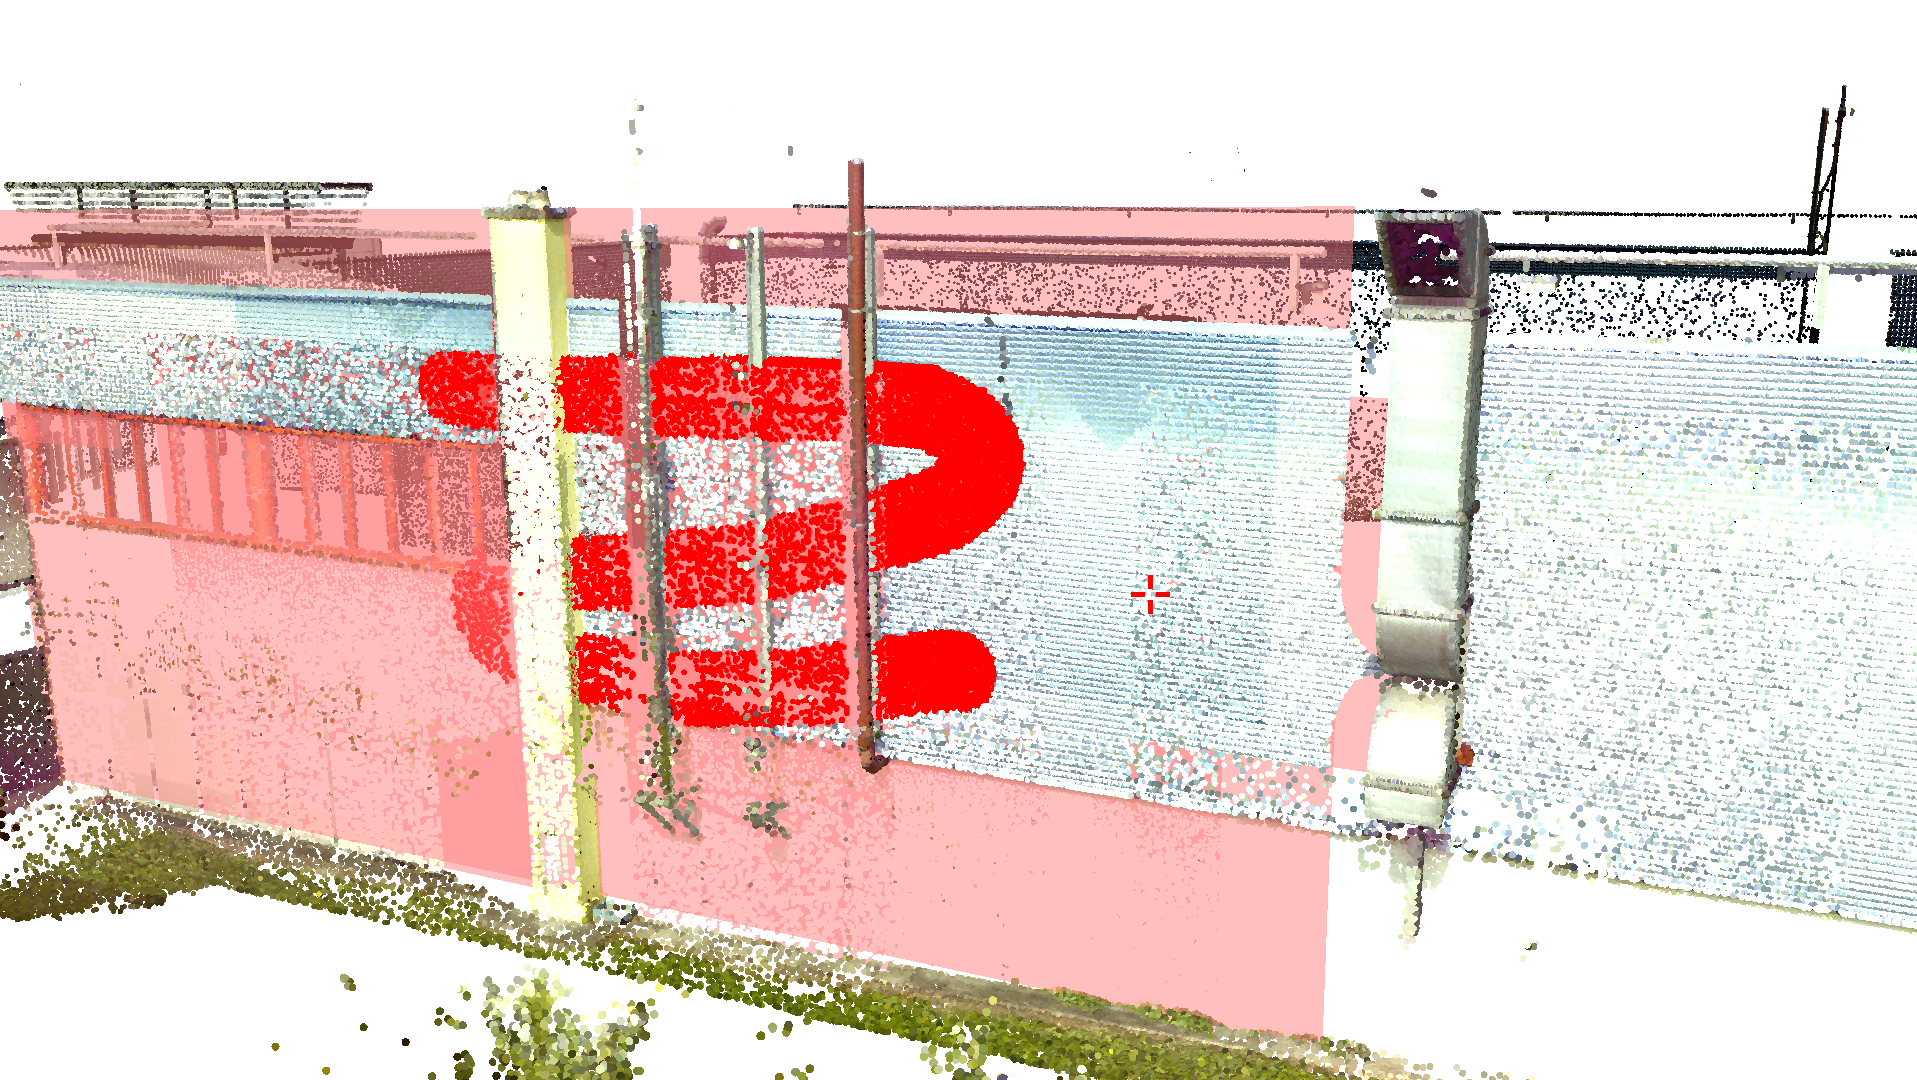
\includegraphics[width=\textwidth]{Results/technologiezentrum_brush2.png}%
  }
\caption[Example of an improved volumetric brush selection]
{A volumetric brush selection is performed on the selected support shape in (a). Points are only selected if they belong to the support shape and intersect the brush. The result of the selection can be seen in (b).}
\label{fig:technologiezentrum_brush}
\end{figure}


\begin{figure}
\centering
\subcaptionbox{ \label{fig:technologiezentrum_lod_increment1}}{%
  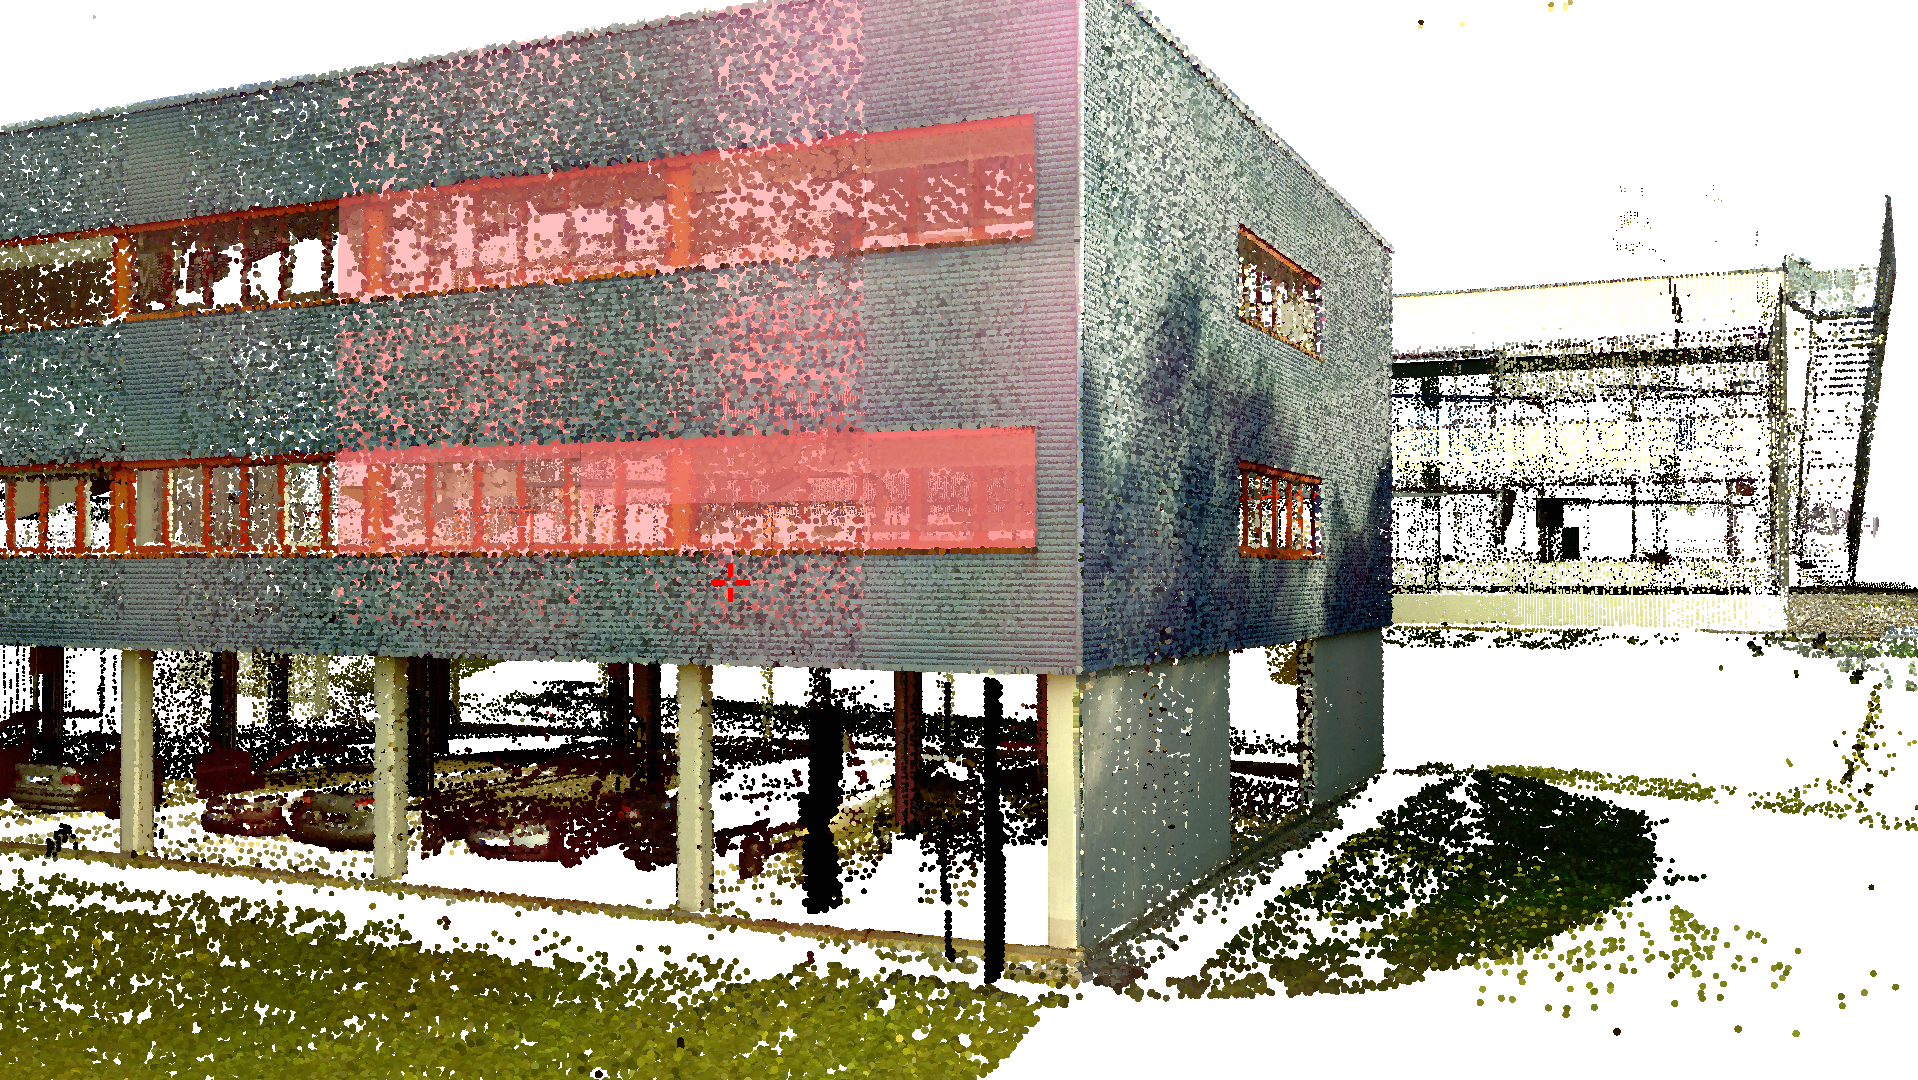
\includegraphics[width=\textwidth]{Results/technologiezentrum_lod_increment1.png}%7
  }
\subcaptionbox{ \label{fig:technologiezentrum_lod_increment2}}{%
  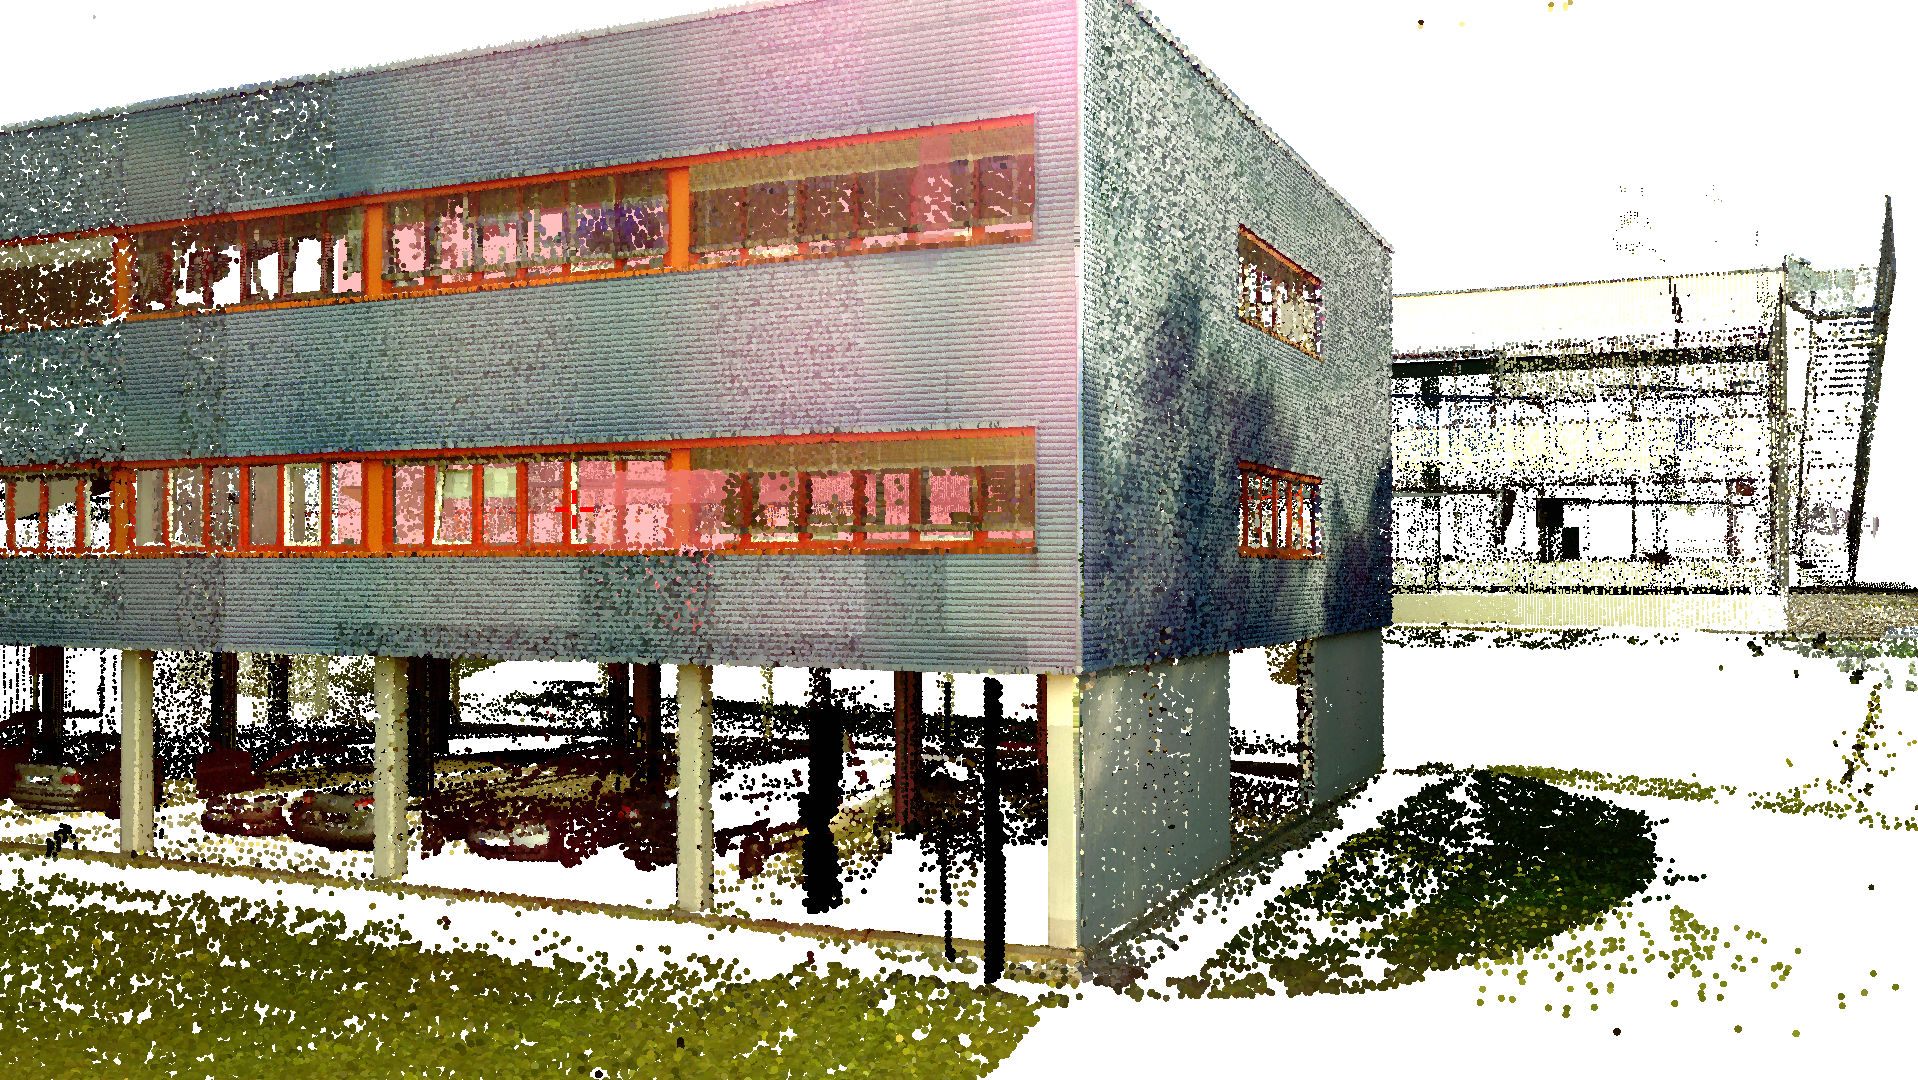
\includegraphics[width=\textwidth]{Results/technologiezentrum_lod_increment2.png}%
  }
\caption[Example of the local increment of level of detail]
{This figure shows the use of the level-of-detail increment interaction. The level of detail is incremented along the selected support shape (drawn in red). (a) shows the original rendering model of the point cloud, (b) shows the point cloud with additional points. }
\label{fig:technologiezentrum_lod_increment}
\end{figure}


\begin{figure}
\centering
\subcaptionbox{ \label{fig:syntheticScene_lasso1}}{%
  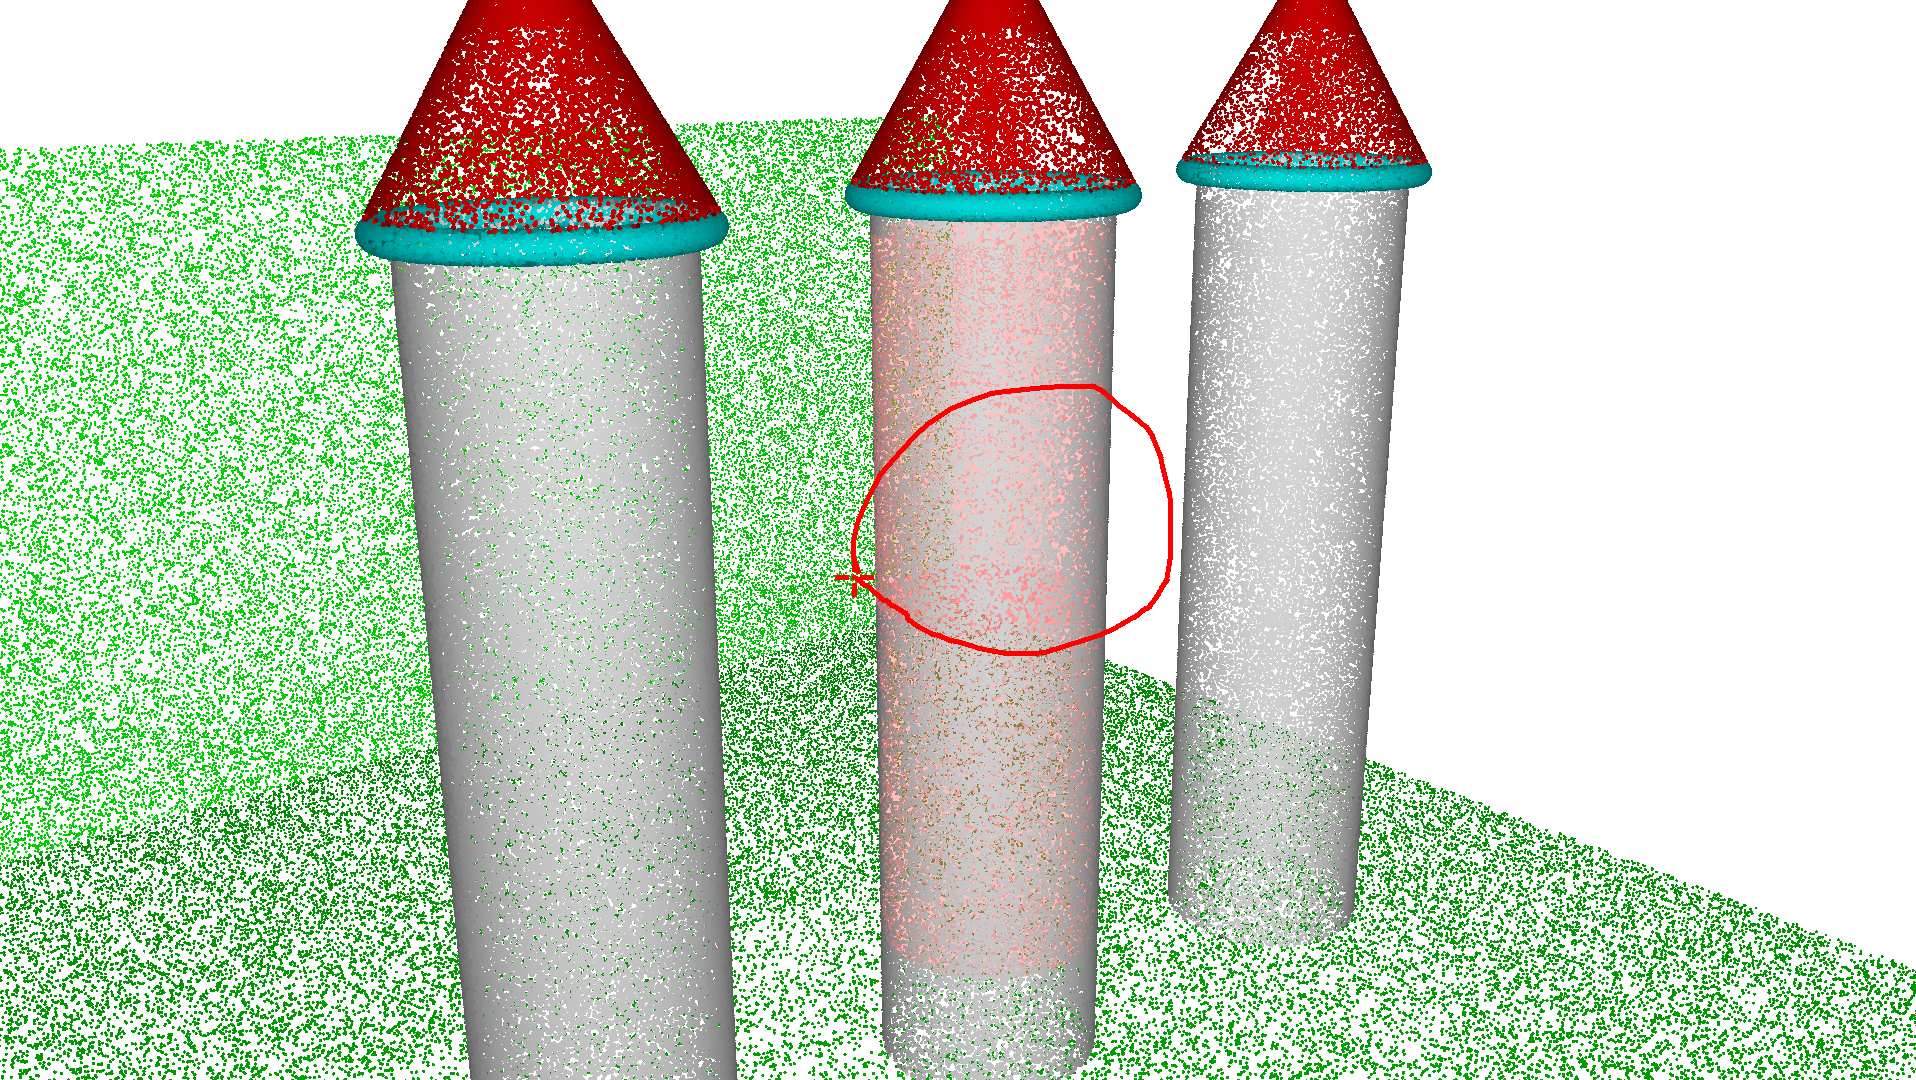
\includegraphics[width=\textwidth]{Results/synthetic_point_cloud_lasso1.png}%7
  }
\subcaptionbox{ \label{fig:syntheticScene_lasso2}}{%
  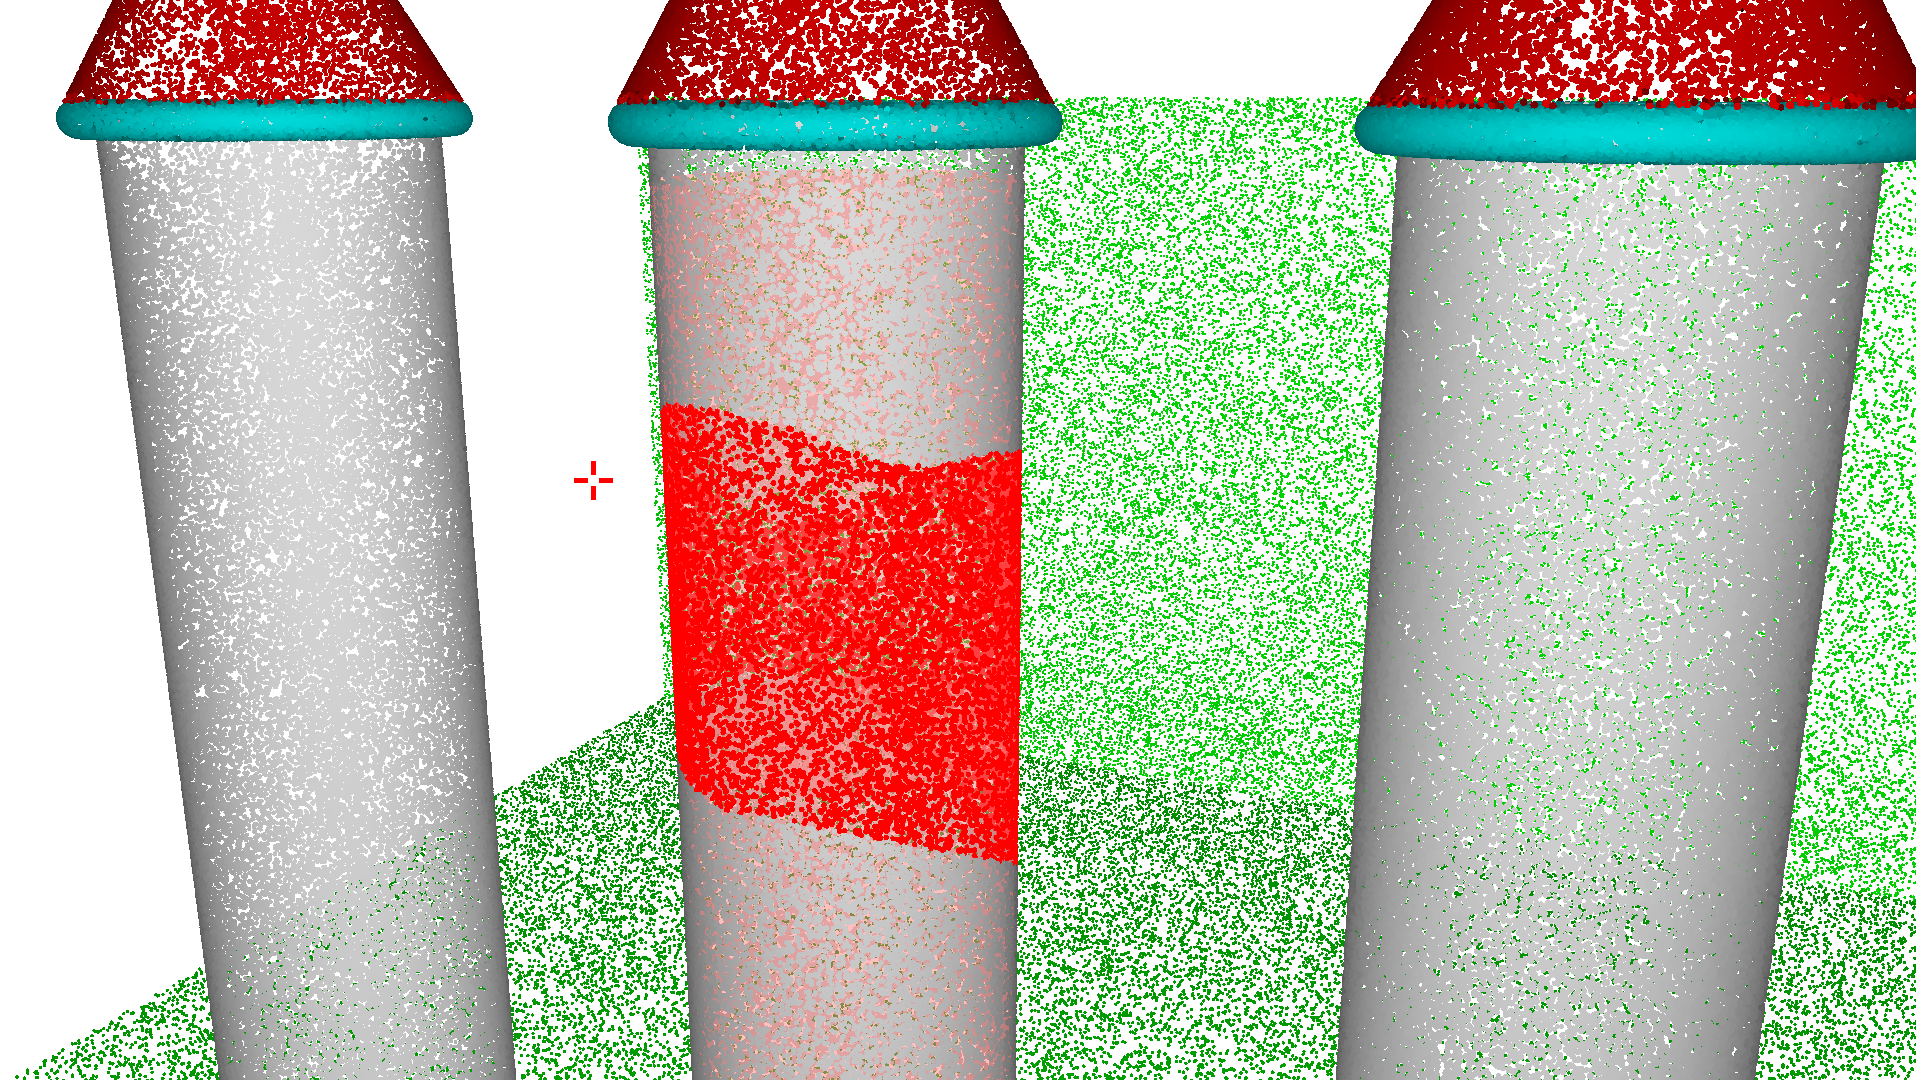
\includegraphics[width=\textwidth]{Results/synthetic_point_cloud_lasso2.png}%
  }
\caption[Example of an improved lasso selection on a cylinder]
{This figure shows an improved lasso selection performed using a cylinder shape as support. (a) shows the lasso that is drawn on the screen, (b) shows the selection result from a different angle. Points in the back of the cylinder are selected, as they are approximated by the cylinder as well. }
\label{fig:synthetic_scene_lasso}
\end{figure}


\begin{figure}
\centering
\subcaptionbox{ \label{fig:syntheticScene_brush1}}{%
  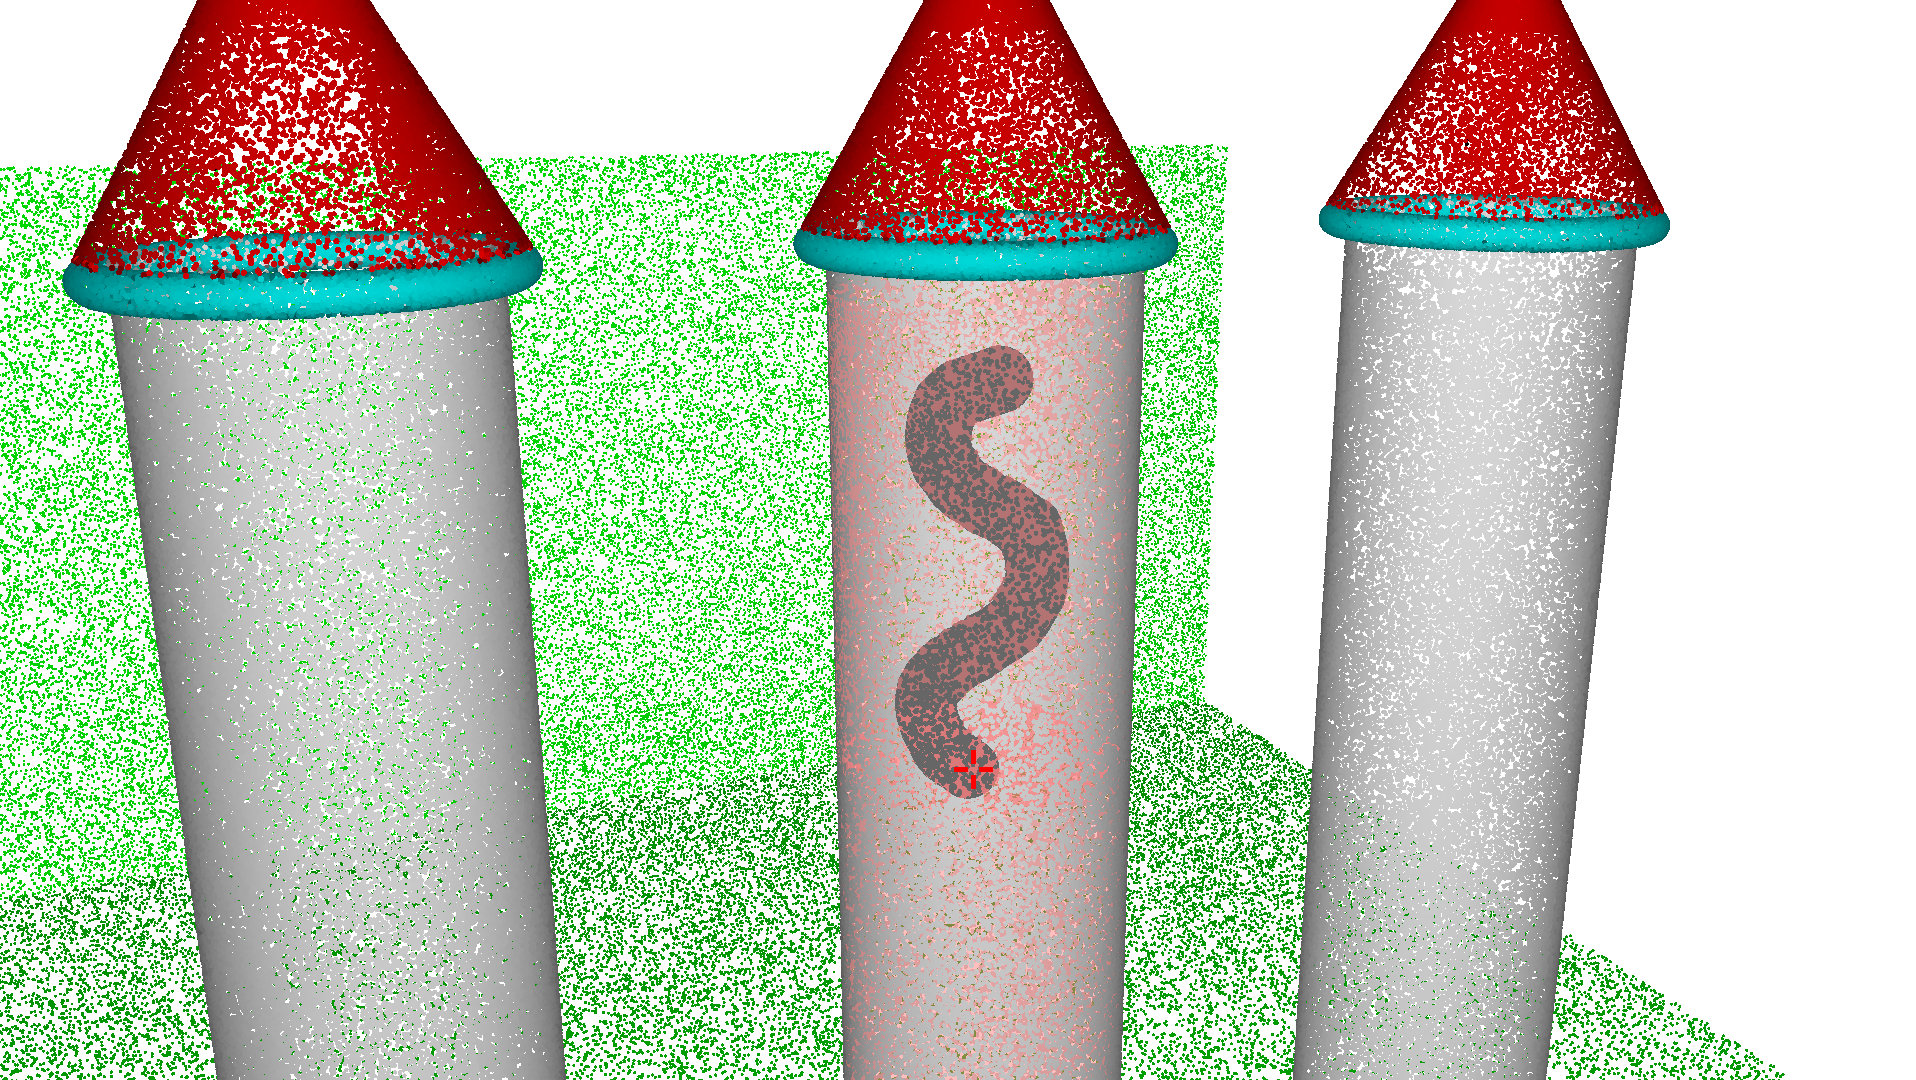
\includegraphics[width=\textwidth]{Results/synthetic_point_cloud_brush1.png}%7
  }
\subcaptionbox{ \label{fig:syntheticScene_brush2}}{%
  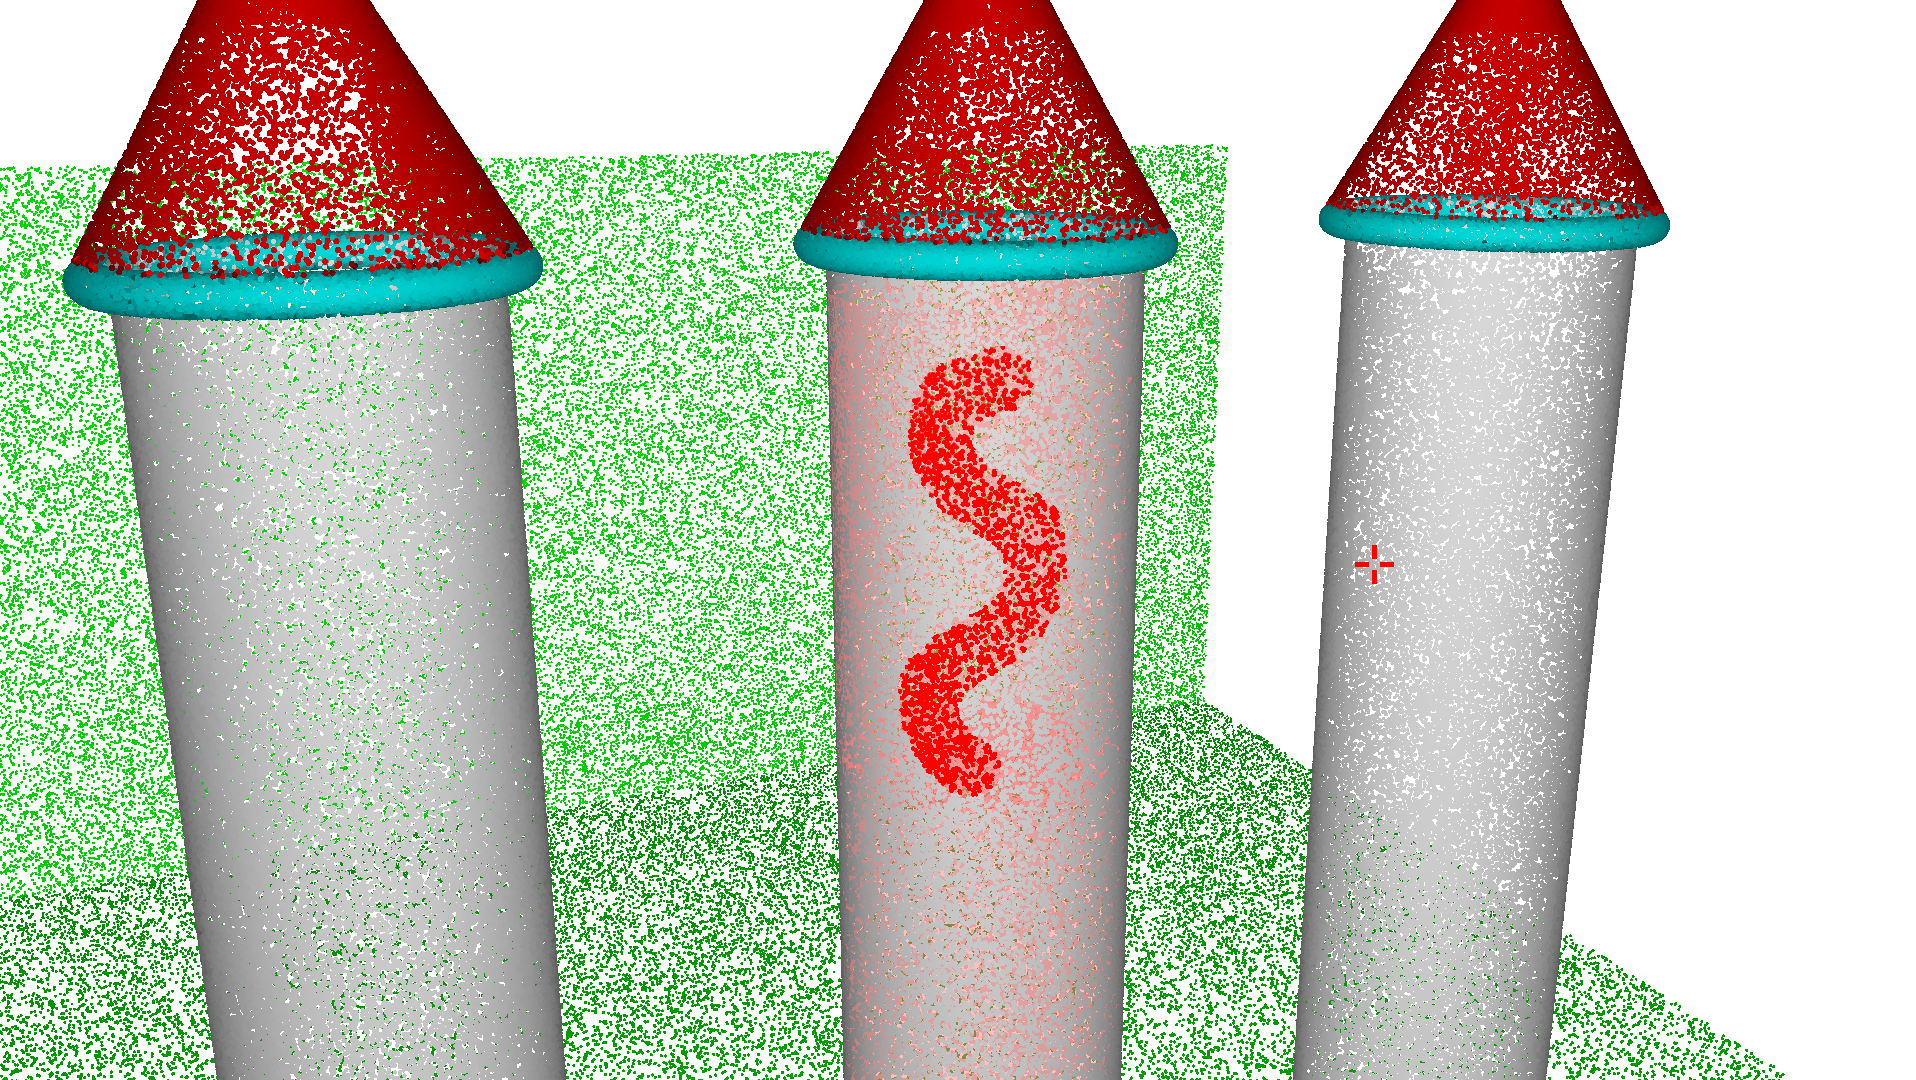
\includegraphics[width=\textwidth]{Results/synthetic_point_cloud_brush2.png}%
  }
\caption[Example of an improved volumetric brush selection on a cylinder]
{This figure shows the volumetric brush selection on a selected cylinder shape. The brush sticks to the side of the cylinder that is facing the camera.}
\label{fig:synthetic_scene_brush}
\end{figure}